This chapter outlines the methods and techniques employed in the development of a conversational question-answering system designed for the use with a collection of documents as knowledge source. The chapter is structured as follows: Section \ref{sec:overview} provides an overview of the desired use case, its objectives, and constraints concerning a Conversational Question Answering System. Section \ref{sec:problem_statement} will introduce the fundamental document inquiry model, and Section \ref{sec:conrag} presents a general framework that can be utilized for the implementation of a Conversational Question Answering System. Its subsections will highlight and discuss the components introduced within the framework. Section \ref{sec:conclusion_contribution} will summarize the contribution of this thesis to the field of Conversational Question Answering Systems.


\section{Overview and Objective}
\label{sec:overview}

The primary use case addressed in this thesis can be summarized as follows: Imagine having a collection of documents, and our goal is to create a chatbot capable of engaging in conversations about the knowledge within these documents. This chatbot provides accurate answers to questions based on the content of the documents and furnishes supporting evidence from these documents. Furthermore, it enables users to have a conversational query experience, allowing them to ask follow-up questions and engage in dialogue with the chatbot based on its previous responses. Figure \ref{fig:use-case} illustrates an example of this use case.

\begin{figure}
    \centering
    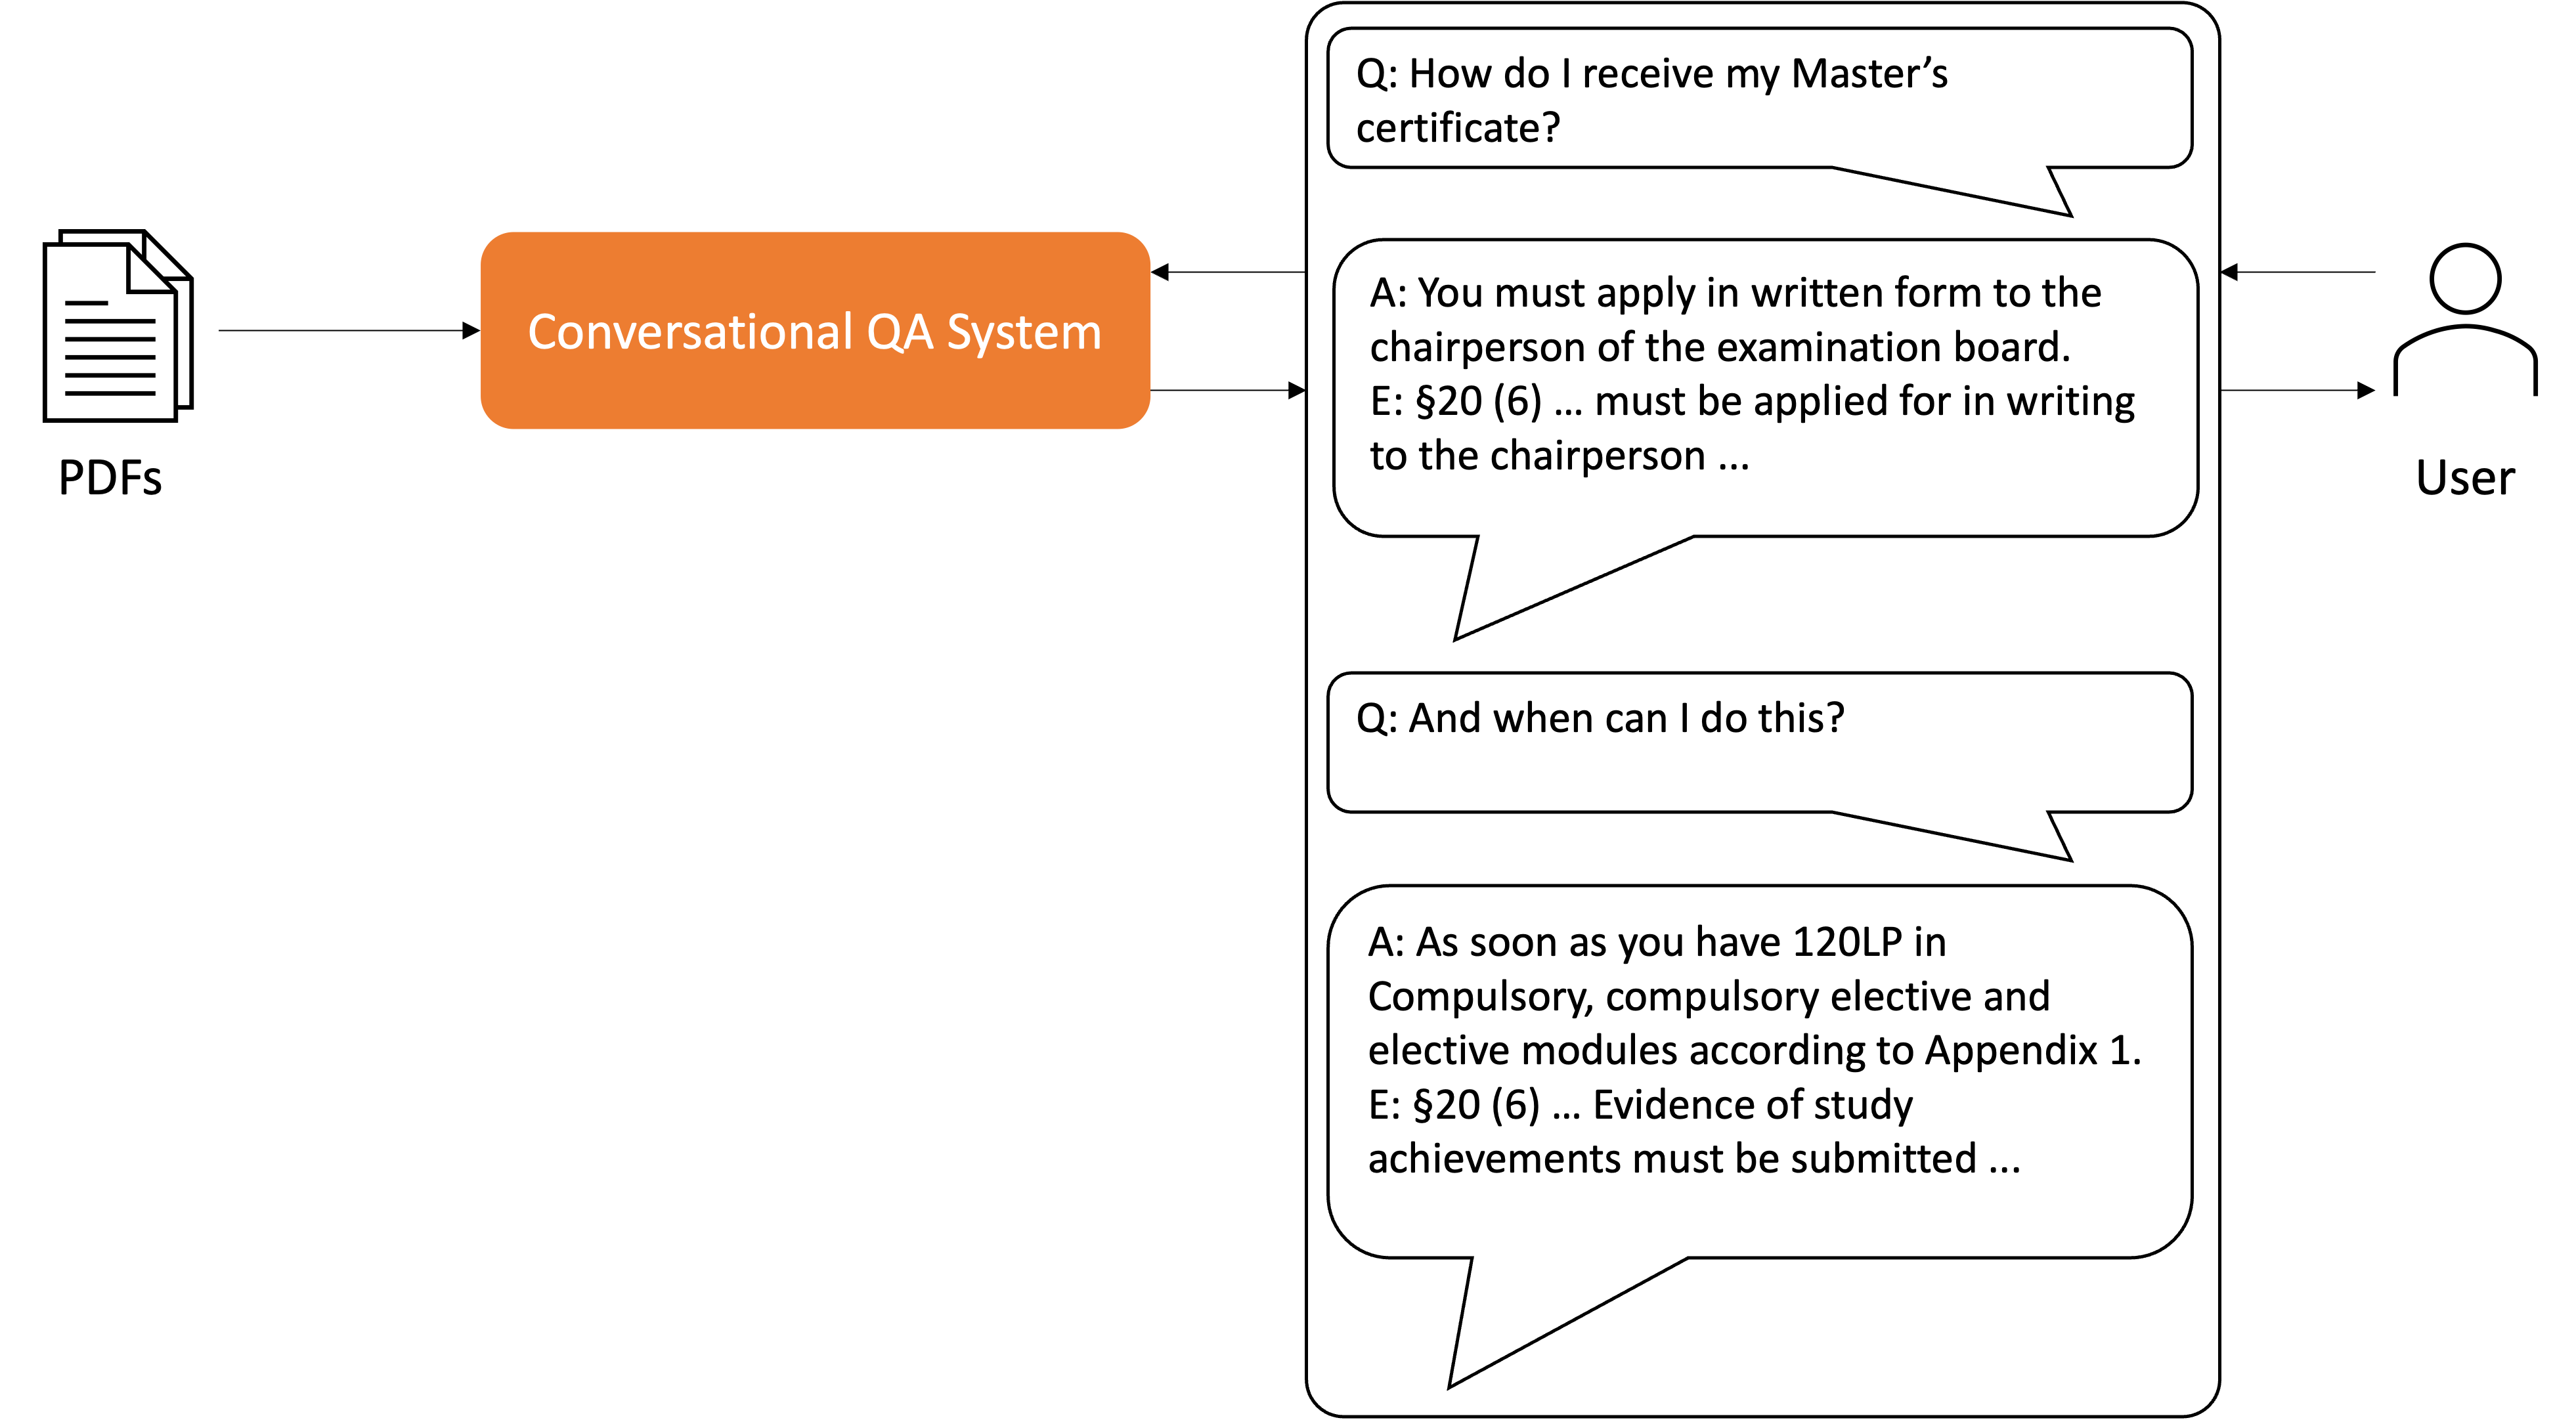
\includegraphics[width=0.8\textwidth]{Grafiken/Use_Case.png}
    \caption{Overview of the Example Use-Case}
    \label{fig:use-case}
\end{figure}

Currently, to the best of our knowledge, there is no scientific paper or similar resource offering a comprehensive framework or pipeline to address this use case. This thesis aims to bridge this gap by presenting a framework and pipeline designed to tackle this specific scenario. Figure \ref{fig:overview-system-architecture} provides an overview of the system architecture. The system follows the \gls{rag} architecture, as detailed in Section \ref{subsec:qa_retrieval}, which extends the classical Retriever-Reader with a \gls{llm} as a Reader, capable of incorporating parametric knowledge. To extend \gls{rag} to a \gls{convqa}, a \gls{cqu} unit, as introduced in Section \ref{subsec:cqa_contextual_query_understanding}, is essential. This novel architecture will be termed \textbf{\glsentrydesc{conrag} (\glsentrytext{conrag})}. The extraction pipeline will be discussed in Section \ref{subsec:extract}, with its primary tasks being the extraction of passages from the provided set of documents, the creation of an index, and the optional generation of synthetic training data. The three major modules comprising the architecture, namely the \textit{Retriever}, \textit{Reader}, and \textit{\gls{cqu}}, will be elaborated in their respective sections: \ref{subsec:retriever}, \ref{subsec:reader}, and \ref{subsec:cqu}.

\begin{figure}
    \centering
    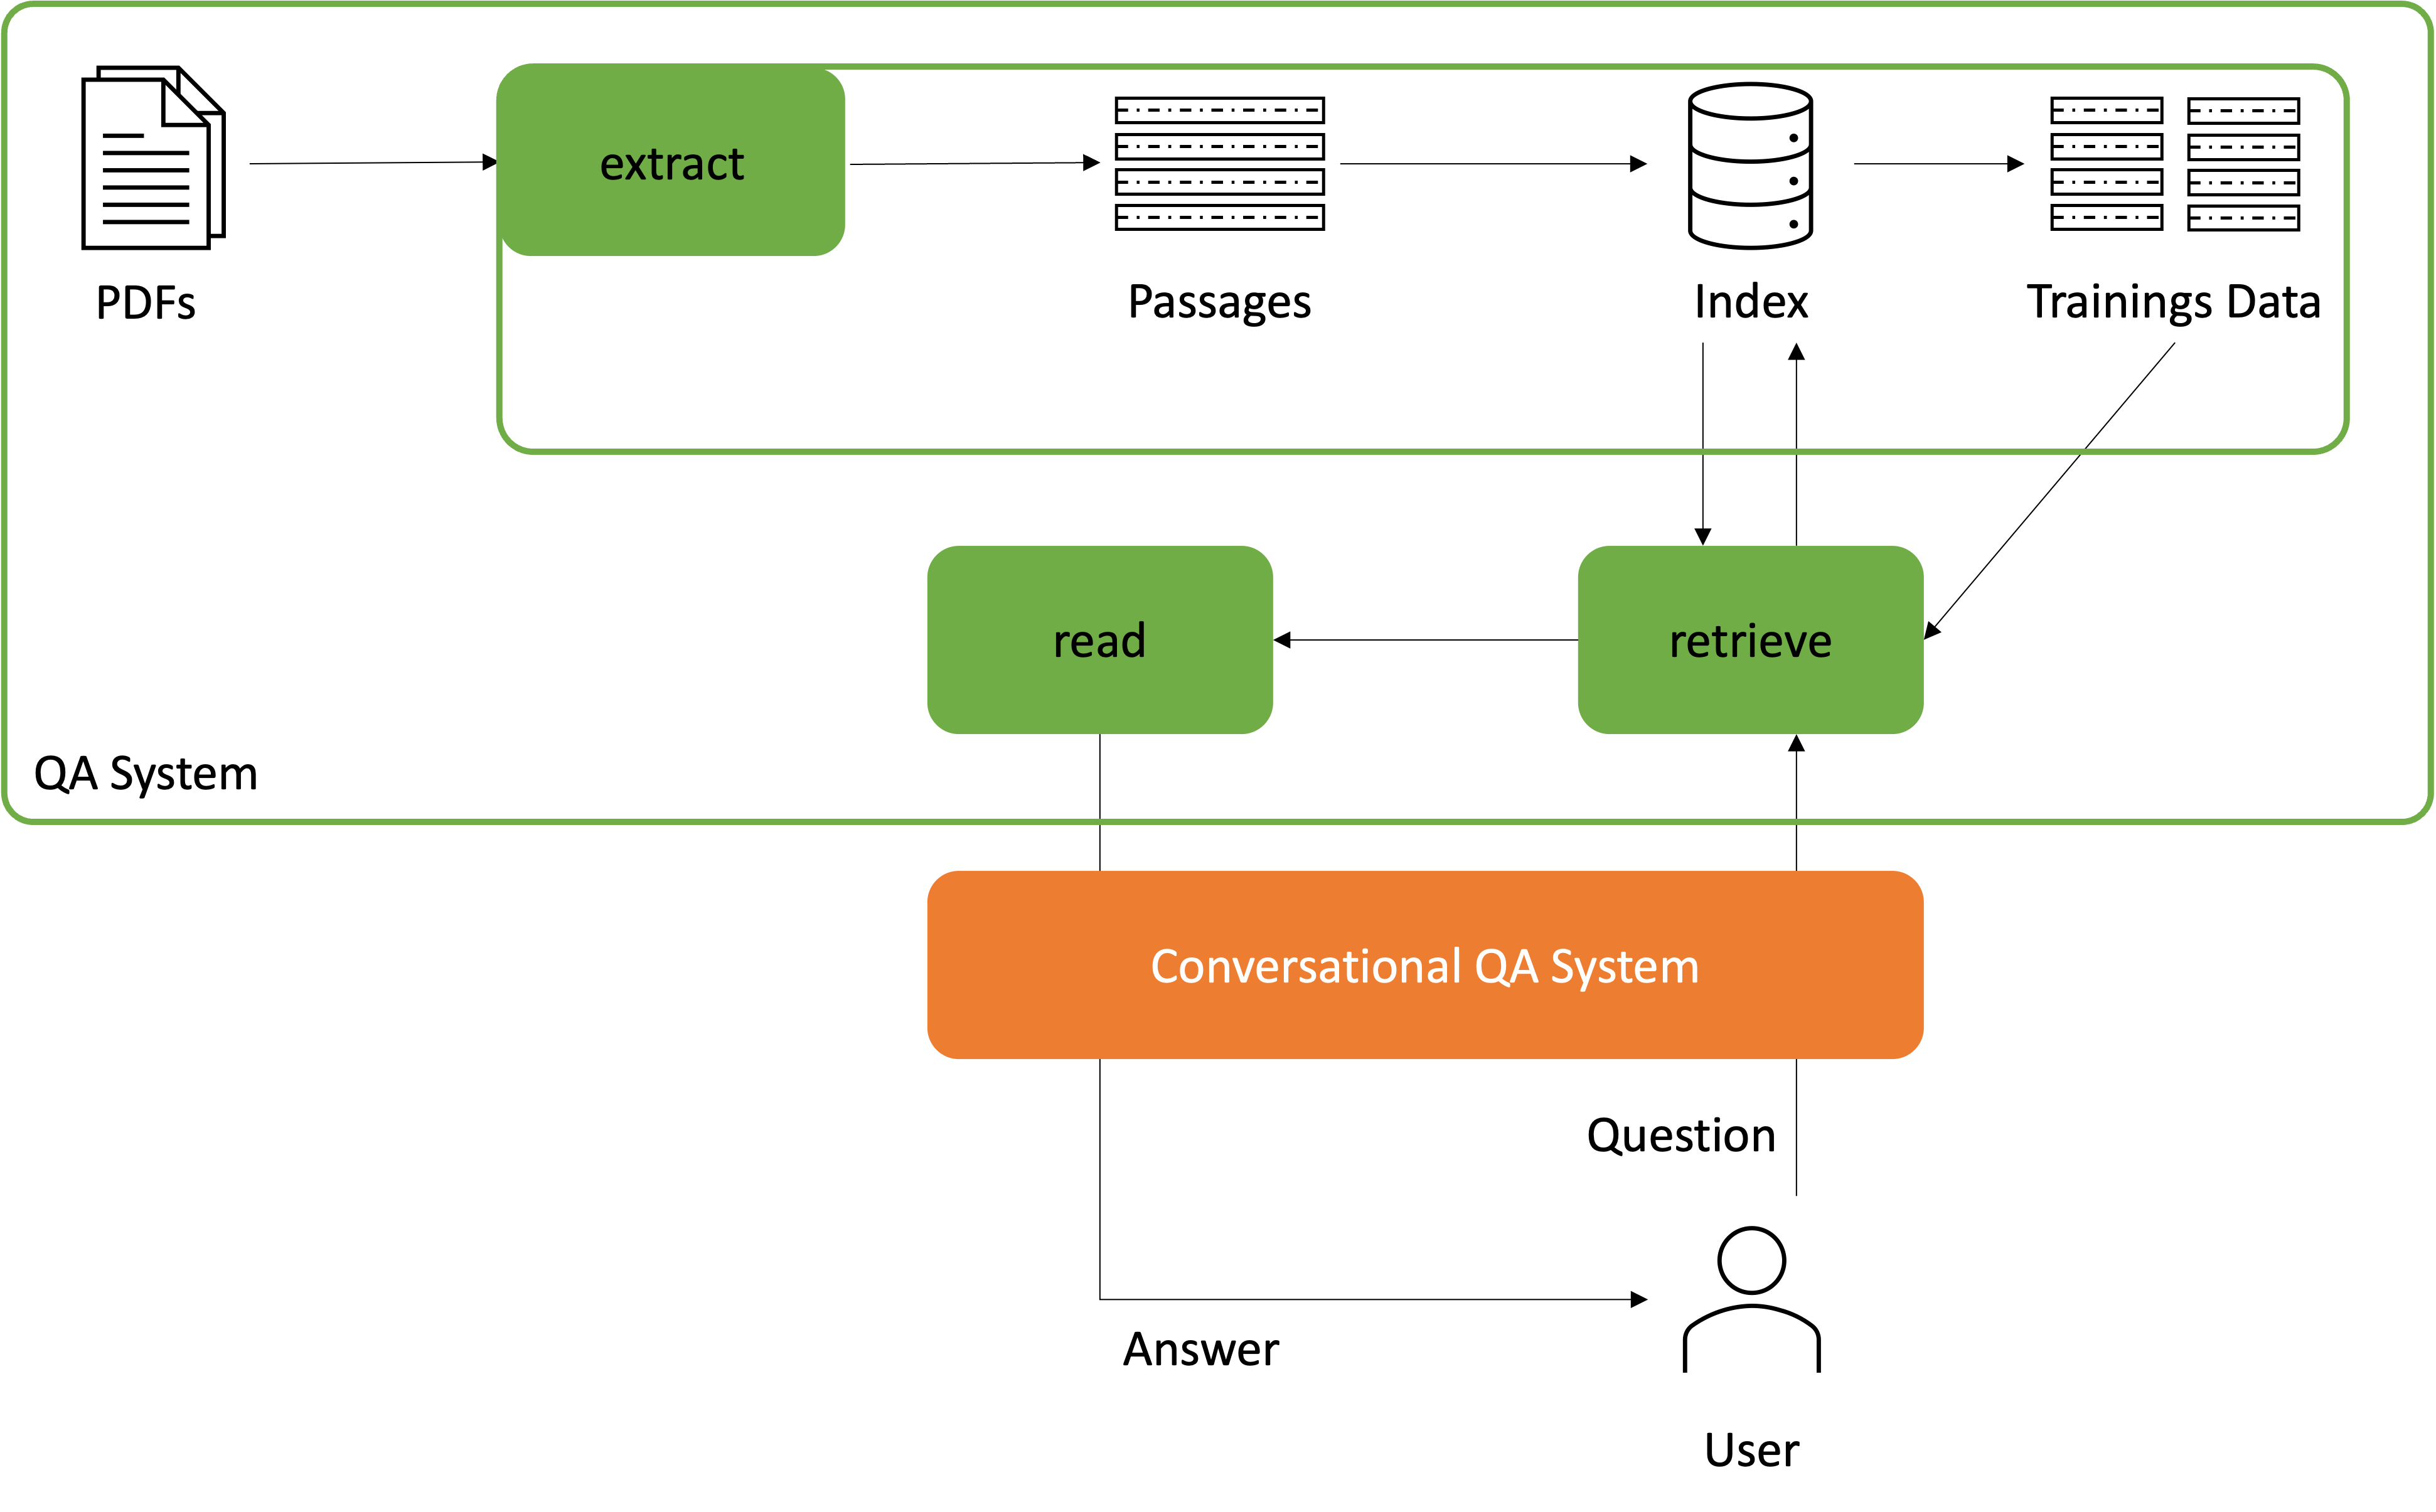
\includegraphics[width=0.8\textwidth]{Grafiken/System_Architecture.png}
    \caption{Overview of the System Architecture}
    \label{fig:overview-system-architecture}
\end{figure}

To summarize, the objectives of the QA capabilities of the system are as follows:

\begin{enumerate}
    \item Utilize \textbf{documents} as the primary \textbf{knowledge source}.
    \item Enable the QA-System to handle a \textbf{variety of answer types}, including: \textbf{extractive}, \textbf{abstractive}, and \textbf{boolean}.
    \item \textbf{Provide references} to document snippets \textbf{as evidence to answers}.
    \item Ensure the pipeline's generalizability by using \textbf{open-domain methods}, allowing it to adapt to new domains or knowledge sources with \textbf{minimal or no supervision} and \textbf{small datasets}.
    \item Design the pipeline to be \textbf{feasible without the need for datacenter-grade hardware resources}, making it accessible for development on standard research hardware.
    \item \textbf{Prioritize accuracy as the primary objective}, as constraining memory consumption is indirectly covered in point (5). \textbf{Latency is not a primary concern}, as the system is not intended for real-time use and will not be optimized for that in this thesis.
\end{enumerate}


Regarding the ConvQA-System, the objectives are as follows:

\begin{enumerate}
    \item Enable the ConvQA-System to \textbf{handle} the following follow-up \textbf{question types: drilling-down, clarification, topic shift} and \textbf{comparison}.
    \item Be able to take Initiative in the form of \textbf{clarifying questions}.
    \item The \textbf{memory} will be \textbf{limited to a session} and not multi-session.
\end{enumerate}

\section{Document Enquiry Model}
\label{sec:problem_statement}

This Section will lay out the problem of document-based \gls{convqa}. 

Substantially the fundamental source of knowledge is \textit{documents}. A \textit{document} can be any type of structured or unstructured file, which is being used for storing and displaying information. Examples are HTML (structured) or PDF (unstructured) files. A \textit{document} consists of content $C_d$, a collection of information units $c_d$, whereas the content $C_d$ has to have at least one $c_d$, but can contain also multiple. On top a \textit{document} contains metadata $M_d$, which are a collection of key-value-pairs, an example is $M_d = \{(title,\text{Examination Regulation Master Data and Computer Science}),\allowbreak (publish\_date \allowbreak, 14.06.2022)\}$. Next to the mentioned components of a \textit{document}, it has also a unique identifier $UID_d$, therefore a \textit{document} $d = (C_d, M_d, UID_d)$. For this thesis we will only consider textual information units in $C_d$ and not figures or images. Out of the necessity, for knowledge granularity and precise information context, we will define \textit{passages} next. A \textit{passage} $p$ is a subsequence of a string of textual content $c_d \in C_d$. The granularity of $p$ can be defined as use-case specific. If $p$ is a sentence, 100 tokens or the full textual content $c_d$. Nevertheless, every $p$ contains a reference to the original document $d$ it was taken from and has its own unique identifier $UID_p$. This leads to the following \textit{Passage Model}:
\begin{definition}
    \textbf{(Passage Model)} A passage $p$ is a subsequence of a textual content string $c_d \in C_d$ of a document $d = (C_d,M_d, UID_d)$, whereas $p = (content, UID_p, UID_d)$.
    \label{def:passage_model}
\end{definition}

Definition \ref{def:passage_model} indicates that the hierarchical or sequential order between passages inside a document won't be captured. This is true for this thesis work only, other approaches may use an incremental index instead of $UID_p$ to indicate the order of passages inside a document $d$.

For ease of notation, we will refer to the \textit{content} of a passage $p$ as $p$ itself in the following. The collection of all \textit{passages} $P$ will be referred to as the \textit{Knowledge Source}. 

For the following definitions, it's important to clarify the concept of \textit{Intent} first. A simple example to illustrate intent is the following:

\begin{quotation}
\noindent Question: When was Barack Obama born? \\\\
Answer 1: 4. August 1961 \\
Answer 2: Barack Obama was the 44th president of the USA. \\
Answer 3: Either 04.08.1961 or 05.09.1962 I'm not sure. 
\end{quotation}

The intent of the question is fulfilled given answer 1, so the answer contains the information the user was looking for when starting the search, but answer 2 misses the search intent. Answer 3 is somewhere in between, as it understands the search intent, but doesn't fulfill it correctly. Therefore intent can be summarized as the user's true information need he had when generating a search query. Mathematically we define intent in the following way:

\begin{definition}
    \textbf{(Intent)} Given two elements, which either can be questions, answers or passages, there exists an operation Intent $\mathcal{I}(x, y)$. This operation returns a value between 0 and 1, which indicates the overlap of the two intents of $x$ and $y$, $\mathcal{I}(x, y) = [0,1]$.
    \label{def:intent}
\end{definition}

Next, we need to define what a \textit{Question} is. For this problem, a question is fundamentally a string. Generally, a question also has an intent, which can be measured against the golden answer (the correct answer to a question). The \textit{Question Model} is therefore defined as follows:

\begin{definition}
    \textbf{(Question Model)} A question $q$ is a string. Given the golden answer $a_q$, $\mathcal{I}(q, a_q) = 1$.
    \label{def:question_model}
\end{definition}

Naturally, where there is a \textit{Question}, there has to be an \textit{Answer}. An \textit{Answer} $a$ is a string, which is the answer to a \textit{Question} $q$. It can be considered a gold answer when $\mathcal{I}(q,a) = 1$. Formally, we define an \textit{Answer} as:

\begin{definition}
    \textbf{(Answer Model)} An answer $a$ is a string, that answers a given question $q$. To which extent answer $a$ answers question $q$ is measured by the \textit{Intent}. If $\mathcal{I}(q,a) = 1$, $a$ is considered a gold answer to $q$.
    \label{def:answer_model}
\end{definition}

In terms of conversations, we split an exchange between two agents into \textit{Turns} as described in Section \ref{subsec:cqa_basics}. Generally speaking, a \textit{Turn} $h$ consists of a tuple $\langle q,a\rangle$, whereas the $a$ is the response to $q$. \textit{Turns} happen in order and therefore have a logical relation. We refer to the sequence of multiple \textit{Turns} within one conversation as \textit{History} $H$.

\begin{definition}
    \textbf{(History Model)} A history $H$ is a seuqnce of turns $h$, whereas $h = \langle q,a\rangle$, $H = \langle h_1, h_2, \dots h_i\rangle$.
    \label{def:history_model}
\end{definition}

As we now have elaborated, what \textit{Questions}, \textit{Knowledge Source}, \textit{Answers} and \textit{History} are, we're ready to define the problem of \gls{convqa}:

\begin{definition}
    \textbf{(Conversational Question Answering Task)} Given a new question $q_{i+1}$ and a history $H = {h_1, h_2, \dots h_i}$, a model ($\mathbf{M}$) generates an answer $a_{i+1}$, based on the provided knowledge in the knowledge source $P$, which satisfies the search intent of $q_{i+1}$. Next to the answer $a_{i+1}$, $\mathbf{M}$ returns $p$ as evidence from $P$. Formally:
    \begin{align*}
        \mathbf{M}: (q_{i+1}, H, P) \rightarrow (a_{i+1}, p)
    \end{align*}
    \label{def:task}
\end{definition}

\section{Conversational Retrieval-Augmented Generation}
\label{sec:conrag}

In order to provide a solution to the Task of \gls{convqa} as defined in Definition \ref{def:task}, the system must be able to perform evidence selection based on a \textit{Knowledge Source} which is an important criterion also laid out in Section \ref{sec:overview}. 

In order to now create a system architecture, that fulfills the task of model $\mathbf{M}$ (see Definition \ref{def:task}), we will split the main task of \gls{convqa} into multiple subtasks:

\begin{enumerate}
    \item \textbf{Information Extraction:} Given a set of documents $D$, extract the textual content $C_d$ of each document $d \in D$ and create a knowledge source $P$ based on $C_d$ of every document $d \in D$.
    \item \textbf{Contextual Query Understanding:} Given a history $H$ and a new question $q_{i+1}$, generate a contextualized question $q_c$ based on $H$, such that $\mathcal{I}(q_c,q_{i+1}) = 1$.
    \item \textbf{Passage Retrieval:} Given a contextualized question $q_c$ and a knowledge source $P$, retrieve the most relevant passages $p$ from $P$ and combine them in an evidence set $E$.
    \item \textbf{Response Generation:} Given a history $H$, a new question $q_{i+1}$ and a set of passages $E$, generate an answer $a$ to $q_{i+1}$ based on $E$, so that $\mathcal{I}(q_{i+1},a) = 1$.
\end{enumerate}

There may exist other approaches to break down the task of $\mathbf{M}$ into sub-tasks, but for this thesis, we will focus on a solution based on the four sub-tasks outlined above. It is to be highlighted, that breaking the task of $\mathbf{M}$ implies also an order in which the sub-tasks have to be performed. Sub-task (1) will be performed once, while (2-4) will be repeated on every new question $q_{i+1}$.

In order to develop a system that can be applied to this abstract task, we match every task to a component. The \textit{Information Extraction} sub-task will be solved by the \textit{Extract} component, further detailed in Section \ref{subsec:extract}. \textit{Passage Retrieval} will be covered by the \textit{Retriever} component, further discribed in Section \ref{subsec:retriever}. The \textit{Response Generation} will be handled by the \textit{Reader} component, more precisely in this thesis we will focus on \gls{llm}s with intrinsic parametric knowledge as \textit{Reader}. This will lead to a \gls{rag} system consisting of the \textit{Retriever} and \textit{Reader}. This choice has been made due to the fact, that the latest research breakthroughs sparked the interest in \gls{rag} systems in comparison to classical Retriever-Reader systems (check therefore the related work Section \ref{sec:related_work}). Details on the \textit{Reader} component will be laid out in Section \ref{subsec:reader}. In order to now handle conversations, a \gls{cqu} unit as described in Section \ref{subsec:cqa_contextual_query_understanding} is necessary to handle the sub-task of \textit{Contextual Query Understanding}. Section \ref{subsec:cqu} will dive into the details.

\begin{figure}
    \centering
    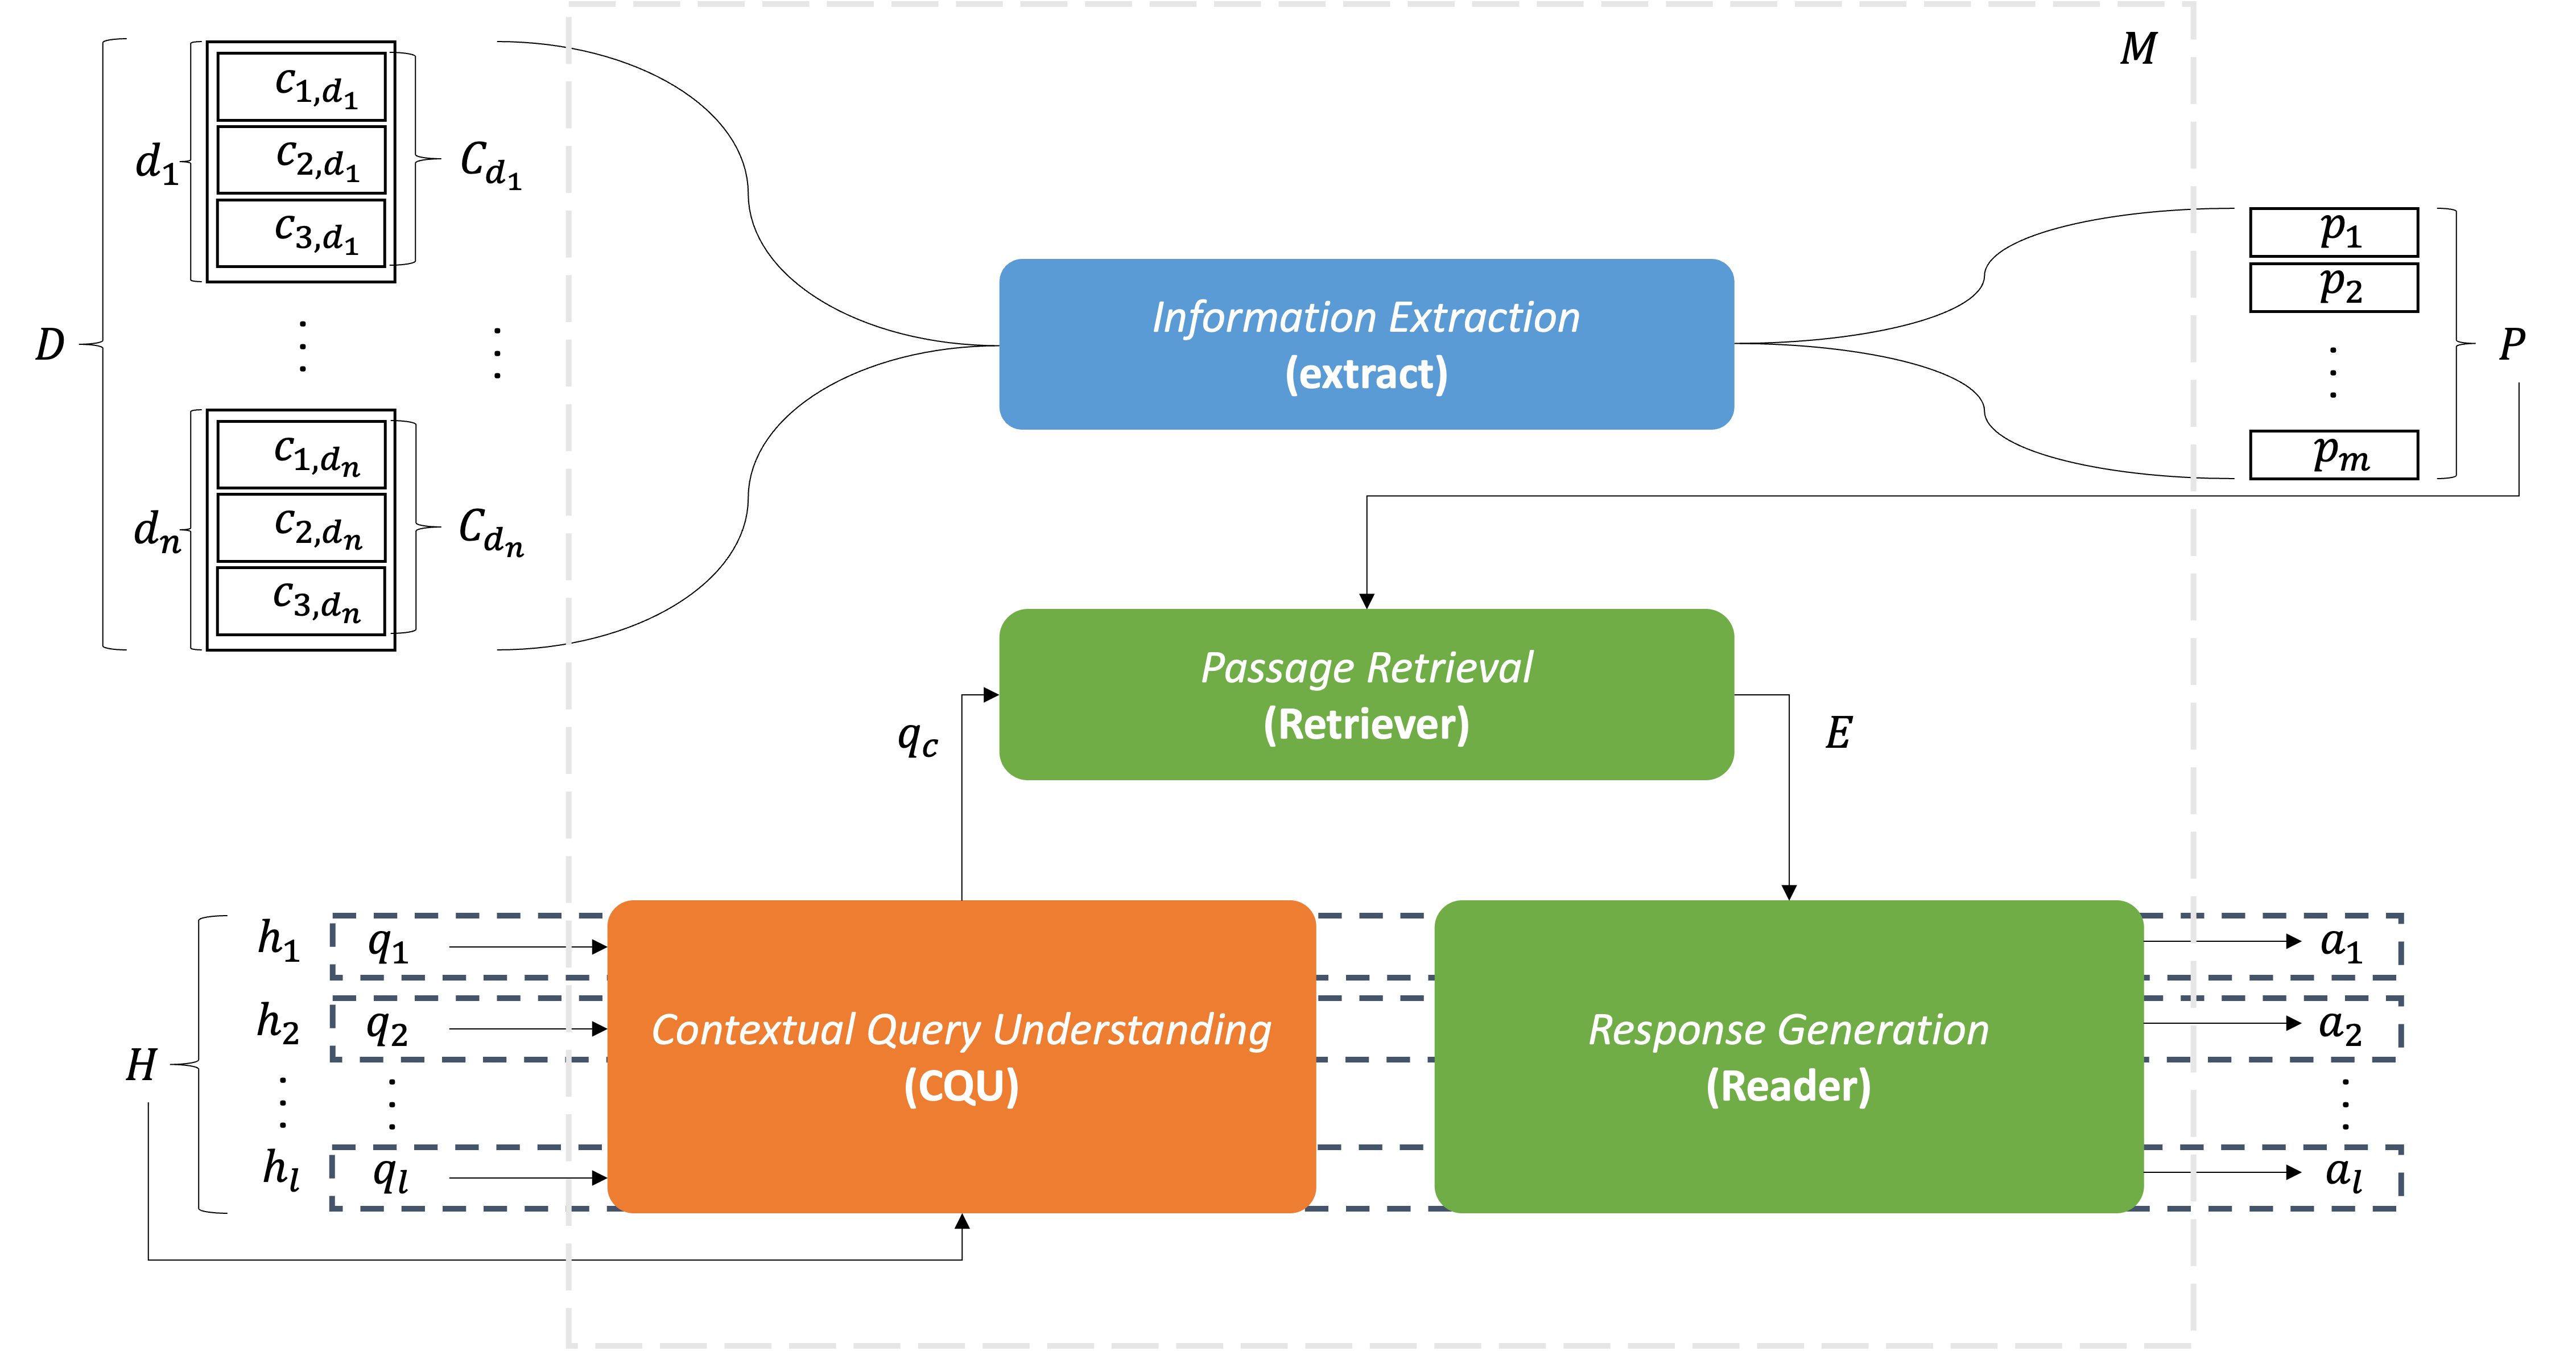
\includegraphics[width=0.8\textwidth]{Grafiken/conrag_konzeptionell.png}
    \caption{Overview of the System Architecture in context of the sub-tasks of $\mathbf{M}$}
    \label{fig:conrag_concept_system_architecture}
\end{figure}

Figure \ref{fig:conrag_concept_system_architecture} illustrates the combination of the four components, which make up the model $\mathbf{M}$ in their corresponding sub-tasks. This is the abstract Model $\mathbf{M}$ which leads, when applied to a real use-case, to the \gls{conrag} system architecture.

% In relation to related work, for some of these sub-tasks, there are already existing components/models, which fullfill this tasks. \textit{Information Extraction} is a well researched field, with many different approaches and models as outlined in Section \ref{subsec:qa_indexing}. Section \ref{subsec:extract} will delve into the details of this sub-task in this context. \textit{Passage Retrieval} and \textit{Response Generation} are commonly implemented as Retriever-Reader Systems as outlined in Section \ref{sec:qa}, nevertheless for this thesis, we will narrow the focus down on \gls{rag} Systems only, as they gained a lot of attention in the last year of research. Details of a both retriever and reader for this specific task will be\textit{Contextual Question Understanding} is a less researched field, with only a few approaches and models.

% This excludes fully generative Models, which can only propose an answer $a$ based on their parametric knowledge. Therefore, the system architecture will have to be based on a Retriever-Reader Architecture. In a Retriever-Reader Architecture, the Retriever identifies important passages $p$ from the knowledge source $P$ given a question $q$ (See Section \ref{subsec:qa_architectures}).

% In the following section, we will outline the general problem field of \gls{convqa}. Unlike other definitions of this problem field, our definition begins with a collection of documents $d \in D$, where \textit{document} refers to any textual knowledge source (e.g., plain text, web pages, etc.). The core task of \gls{convqa} can be defined as follows:

% \begin{definition}
%     \textbf{(\gls{convqa} Task)} The task comprises (i) information extraction, (ii) passage retrieval, (iii) response generation, and (iv) question understanding.
%     \label{def:task}
% \end{definition}

% The system architecture \gls{conrag}, introduced in Section \ref{sec:overview} (see Figure \ref{fig:convqa_system_architecture}), divides these four tasks among four components. Each of these sub-tasks corresponds to a different mechanism of the model ($M$), which is designed to engage in a conversation with a user over a collection of documents $D$. The first task (i) of extraction can be defined as follows:

% \begin{definition}
%     \textbf{(extraction)} An extraction model ($Ext$) is a model which extracts passages from a collection of documents $D$.
%     \begin{align*}
%         \mathbf{Ext: D \rightarrow P}
%     \end{align*} 
%     Whereas $P$ is a set of passages $p \in P$ and $\forall d \in D, \exists p \in P : p \subseteq d$.
%     \label{def:extraction}
% \end{definition}

% Therefore, the input to the next component of $M$, the Retriever $p_\eta(p|q)$, is as follows:

% \begin{equation}
%     \text{Input} = (Q, P) :
%     \begin{cases}
%         \begin{aligned}
%             &\text{question}, && Q = \{q_1, \ldots, q_m\} \\
%             &\text{knowledge source}, && P = \{p_1, \ldots, p_n\}
%         \end{aligned}
%     \end{cases}
% \end{equation}

% This means that the input is a tuple $(Q,P)$ consisting of a set of questions $Q = \{q_1, q_2, \ldots, q_m\}$ and a knowledge source $P = \{p_1, p_2, \ldots, p_n\}$. Therefore, the task of $p_\eta(p|q)$ with parameters $\eta$ can be defined as follows:

% \begin{definition}
%     \textbf{(Passage Retrieval)} A retrieval model ($p_\eta(p|q)$) is a model that generates a relevance score for every tuple $(q,p)$.
%     \begin{align*}
%         \mathbf{p_\eta(p|q) = Score(q,p)}
%     \end{align*}
%     Here, $q$ itself is a tuple $(q,i)$, where $i \in I$, and $I$ is the set of all possible search intents. 
%     \label{def:retrieval}
% \end{definition}

% The set of search intents $I$ (e.g., extractive, abstractive, etc., see Section \ref{subsec:cqa_basics}) is finite. The index $i$ of a question $q$ is implicit and therefore not further specified in the following notations. Hence, instead of representing the whole tuple as $(q,i)$ for each question, we simplify it to just $q$. Task (iii) of response generation is carried out by a generator/reader $p_\theta(a|q,p)$ with parameter $\theta$:

% \begin{definition}
%     \textbf{(Response Generation)} A generation model ($p_\theta(a|q,p)$) is a model that generates an answer $a$ given a question $q$ and top-$k$ retrieved passages $p$.
%     \begin{align*}
%         \mathbf{p_\theta(a|q,p) = a}
%     \end{align*}
%     \label{def:generation}
% \end{definition}

% In a more general context, we assume that there always exists a correct answer $a$ to a question $q$ that can be extracted from the passages $P$. Therefore, we distinguish the following cases:

% \begin{equation}
%     \forall q \in Q, \exists! a \in A : a = 
%     \begin{cases}
%         \begin{aligned}
%             &1. \text{ } f(q, \emptyset), \text{ } &\text{if there is no evidence in } P \\
%             &2. \text{ } f(q, p), \text{ } &\text{if there is exactly one piece of evidence in } P \\
%             &3. \text{ } f(q, E) \mid E \subset P, \text{ } &\text{if there are multiple pieces of evidence in } P
%         \end{aligned}
%     \end{cases}
% \end{equation}

% In case 1, the answer $a$ to the question $q$ indicates that there is no evidence available for this question. Depending on the specific question $q$ intend $i$, this can lead to different answers. Case 2 can be an example of a common extraction question $q$ where the answer $a$ refers to an exact span in one passage $p$. Case 3 involves more complex questions $q$ that require information from multiple passages $p$ to be answered correctly.

% Lastly, task (vi) is handled by a \gls{cqu} $p_\xi(q_c|H,q_i)$ with parameter $\xi$:

% \begin{definition}
%     \textbf{(Question Understanding)} A question understanding model ($p_\xi(q_c|H,q_i)$) is a model that generates a contextualized question $q_c$ given a history $H$.
%     \begin{align*}
%         \mathbf{p_\xi(q_c|H, q_i) = q}
%     \end{align*}
%     Contextualized refers to identifying language-specific features between turns of a conversation to incorporate the context of the conversation into the question $q_i$.
%     \label{def:question_understanding}
% \end{definition}

% The history $H$ is further described in Section \ref{subsec:cqa_basics}.

% Figure \ref{fig:task_convqa} illustrates the general task of \gls{convqa}. It displays the relationship between questions, answers, documents, and the model $M$ on a high level. The following sections will delve deeper into the individual components of $M$. Section \ref{subsec:extract} will discuss sub-task (i), Section \ref{subsec:retriever} will discuss sub-task (ii), Section \ref{subsec:reader} will focus on sub-task (iii), and Section \ref{subsec:cqu} will explore sub-task (vi).

% \begin{figure}
%     \centering
%     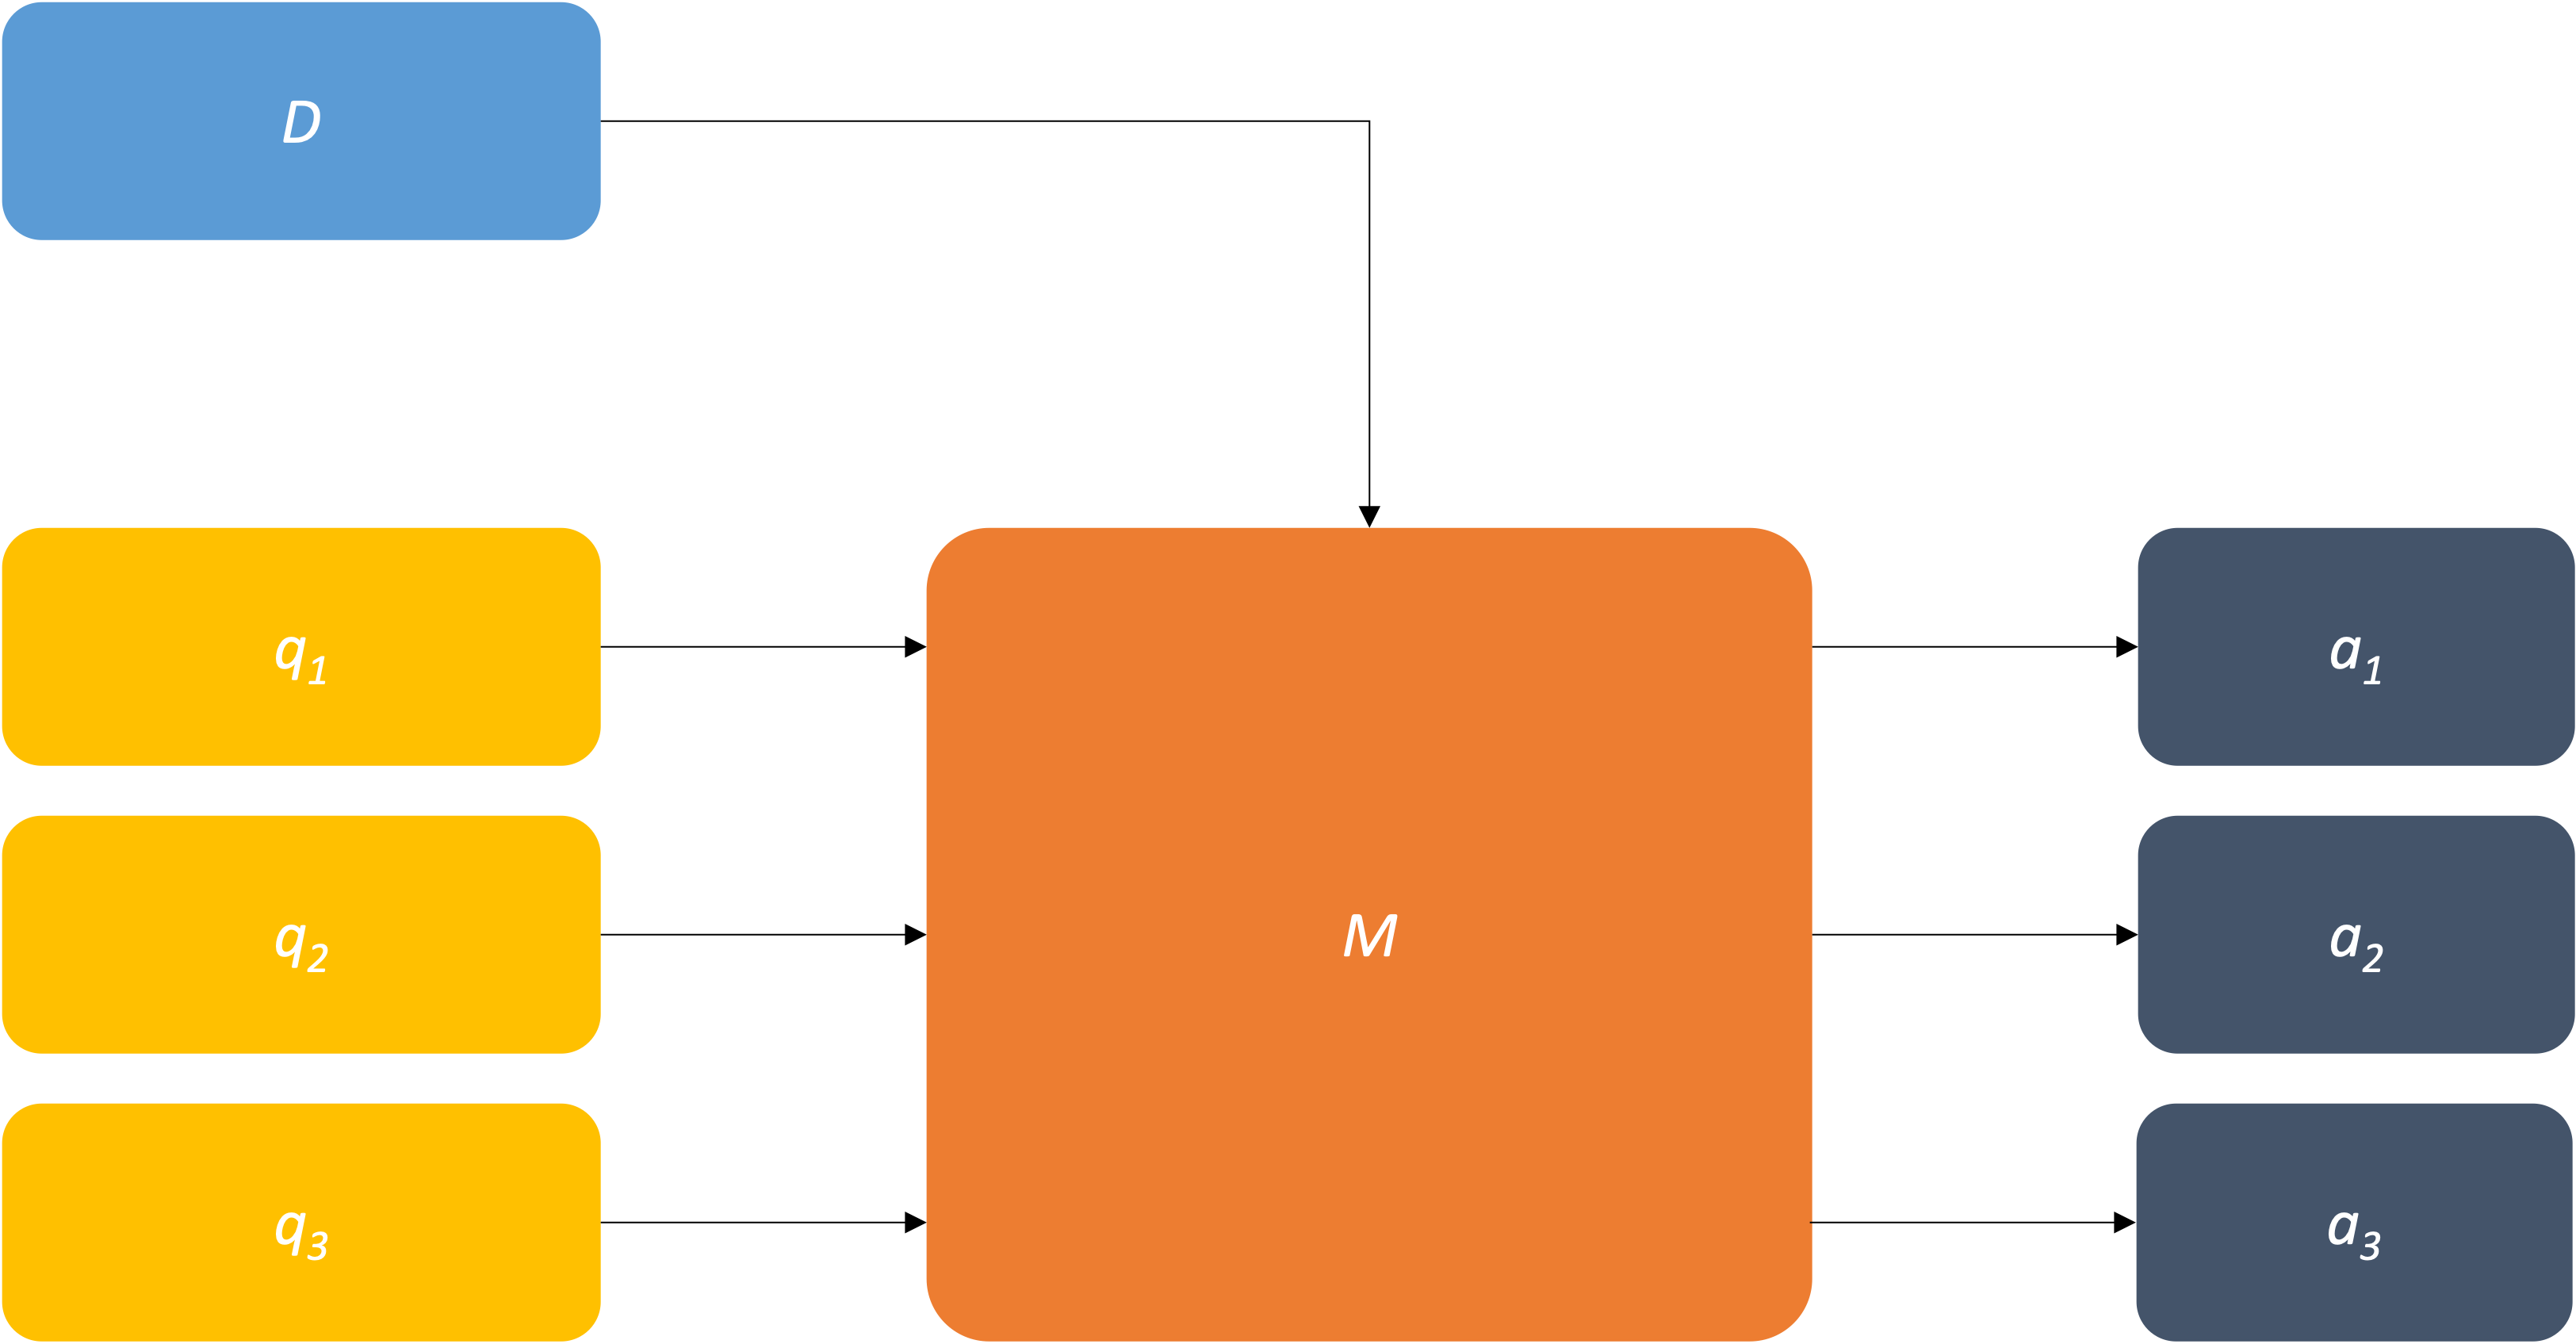
\includegraphics[width=0.8\textwidth]{Grafiken/general_conqa.png}
%     \caption{General Task of \gls{convqa}}
%     \label{fig:task_convqa}
% \end{figure}


% As illustrated in Figure \ref{fig:overview-system-architecture}, it is logical to partition the extensive grid of possibilities into smaller, manageable components that can be explored and designed independently. Consequently, the framework will be divided into two main segments: the extraction pipeline, with its potential configurations outlined in Figure \ref{fig:extract_pipeline}, and the three major modules: Retriever, Reader, and \gls{cqu}, showcasing their possible implementations in Figure \ref{fig:all_components_conrag}.

% \begin{figure}
%     \centering
%     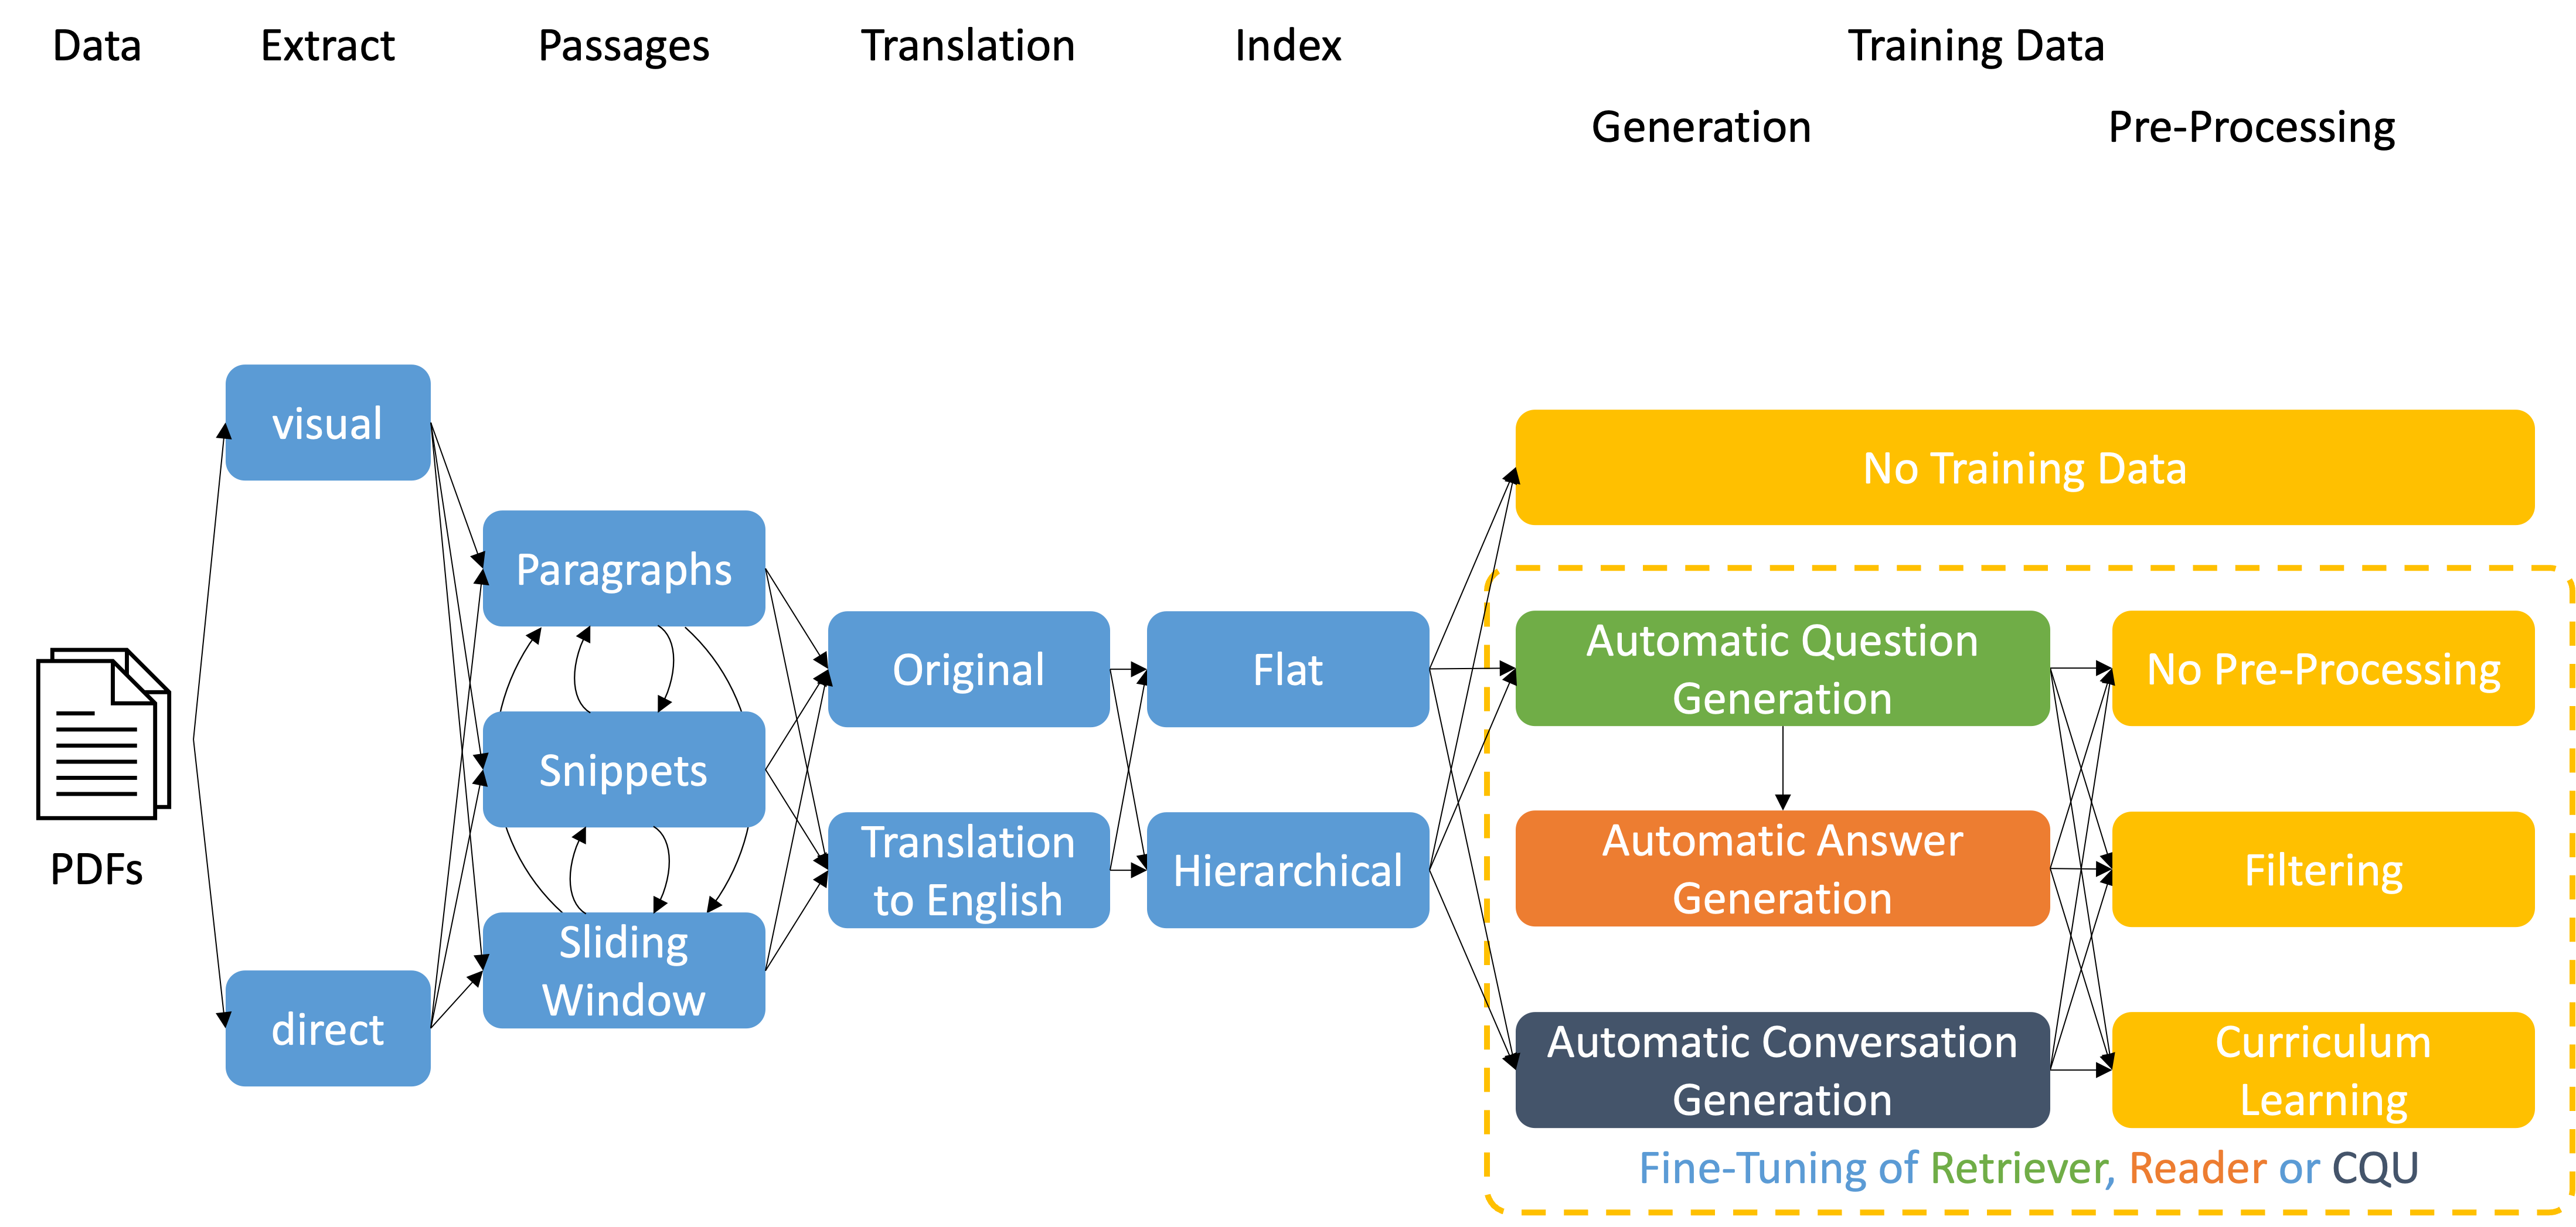
\includegraphics[width=\textwidth]{Grafiken/extract_pipeline.png}
%     \caption{Overview of the Extraction Pipeline Framework}
%     \label{fig:extract_pipeline}
% \end{figure}

% The framework varies in its level of granularity, shifting between high-level concepts and precise details. This is primarily due to the fact that certain aspects of the framework are well-researched and represent state-of-the-art knowledge, while others are ongoing research and necessitate a more abstract, conceptual treatment. For instance, \textit{BM25} is mentioned specifically as the state-of-the-art Sparse Retriever within the Retriever Module, whereas \textit{Automatic Question Generation} in the Training Data Generation step of the extraction pipeline is presented as a high-level concept.

% The framework strives to maintain a high level of generality, intentionally avoiding the incorporation of restrictive paradigms, except for the specified system architecture of \gls{rag} for \gls{qa}. This decision is motivated by the breakthroughs and extensive research endeavors within the field of \gls{llm}s, as exemplified by the exceptional success of \textit{ChatGPT}. In response to the limitations of ChatGPT, including \textit{hallucination}, \textit{implicit knowledge}, and \textit{static knowledge}, interest has surged in the \gls{rag} architecture as a means to address these issues. Presently, there is no existing survey or similar resource that provides a quantitative evaluation of the ongoing business initiatives aimed at implementing RAG-based Systems. Nonetheless, both Google Cloud Services \cite{noauthor_generative_nodate} and Amazon Web Services \cite{noauthor_quickly_2023} have introduced new services that empower customers to construct \gls{rag}-based systems, with Langchain serving as the Framework for the Reader Implementation \cite{noauthor_langchain-ailangchain_nodate}. Consequently, the framework presented here seeks to illuminate potential pathways for implementing a \gls{conrag} system, as depicted in Figure \ref{fig:convqa_system_architecture}, tailored to the use case described in Section \ref{sec:overview}.

% The extraction pipeline can be visualized as a tree, where following different paths signifies making decisions with corresponding implications for subsequent steps and components. In Figure \ref{fig:all_components_conrag}, each column represents a decision to be made, although in some cases, choosing not to decide is itself a decision. Dotted lines encircling multiple frames indicate that a combination or ensemble approach is possible. For a better understanding of how to apply this framework to create a potential system implementation, refer to the example in Figure \ref{fig:example_decission_tree}. As previously mentioned, the framework does not prescribe specific models (e.g., BERT, PaLM, etc.) but rather conceptual approaches (e.g., Cross-Encoder). The example in Figure \ref{fig:example_decission_tree} represents a simple zero-shot baseline, which will also be implemented and tested in this thesis Chapter \ref{chap:eval}.

% \begin{figure}
%     \centering
%     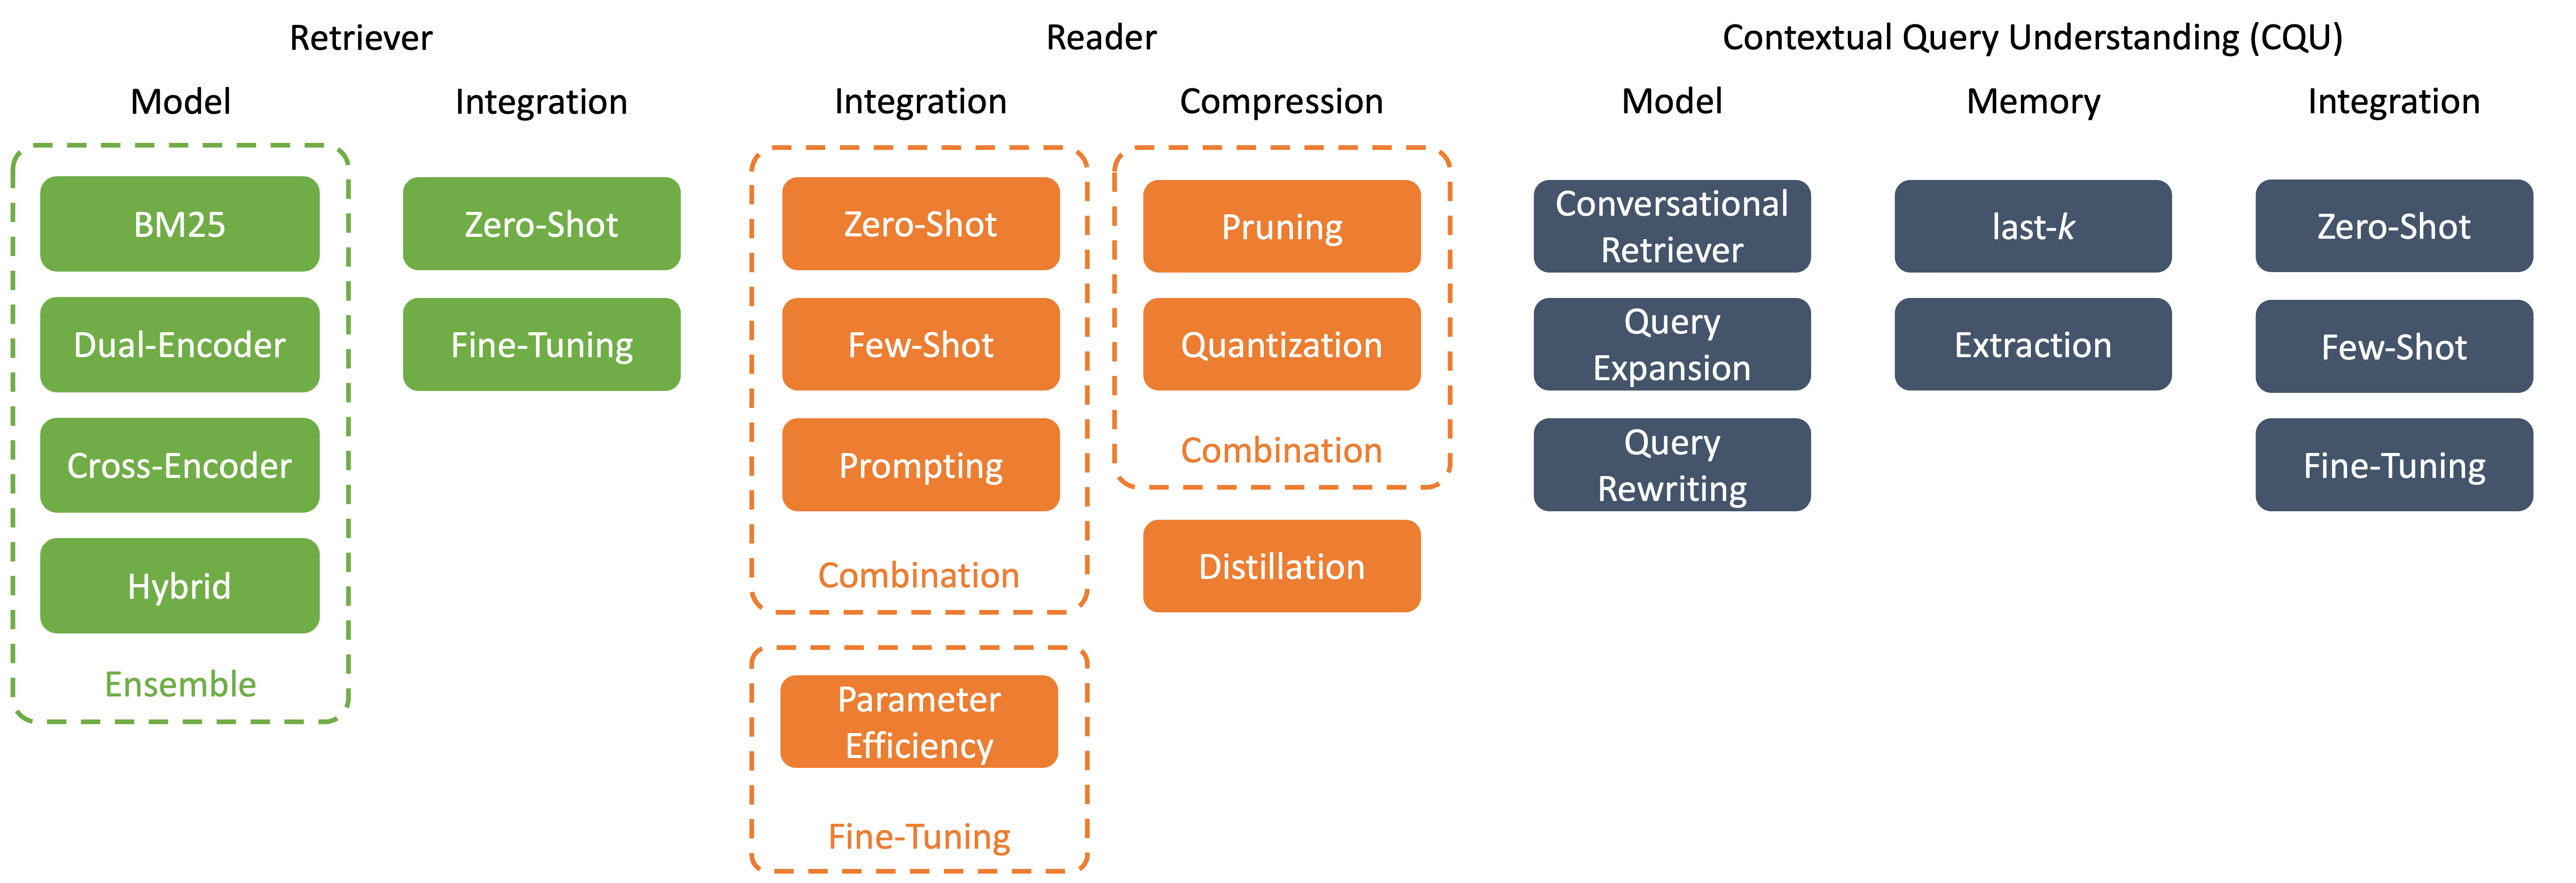
\includegraphics[width=\textwidth]{Grafiken/all_components_conrag.png}
%     \caption{Overview of all Modules of the Framework}
%     \label{fig:all_components_conrag}
% \end{figure}

% \begin{figure}
%     \centering
%     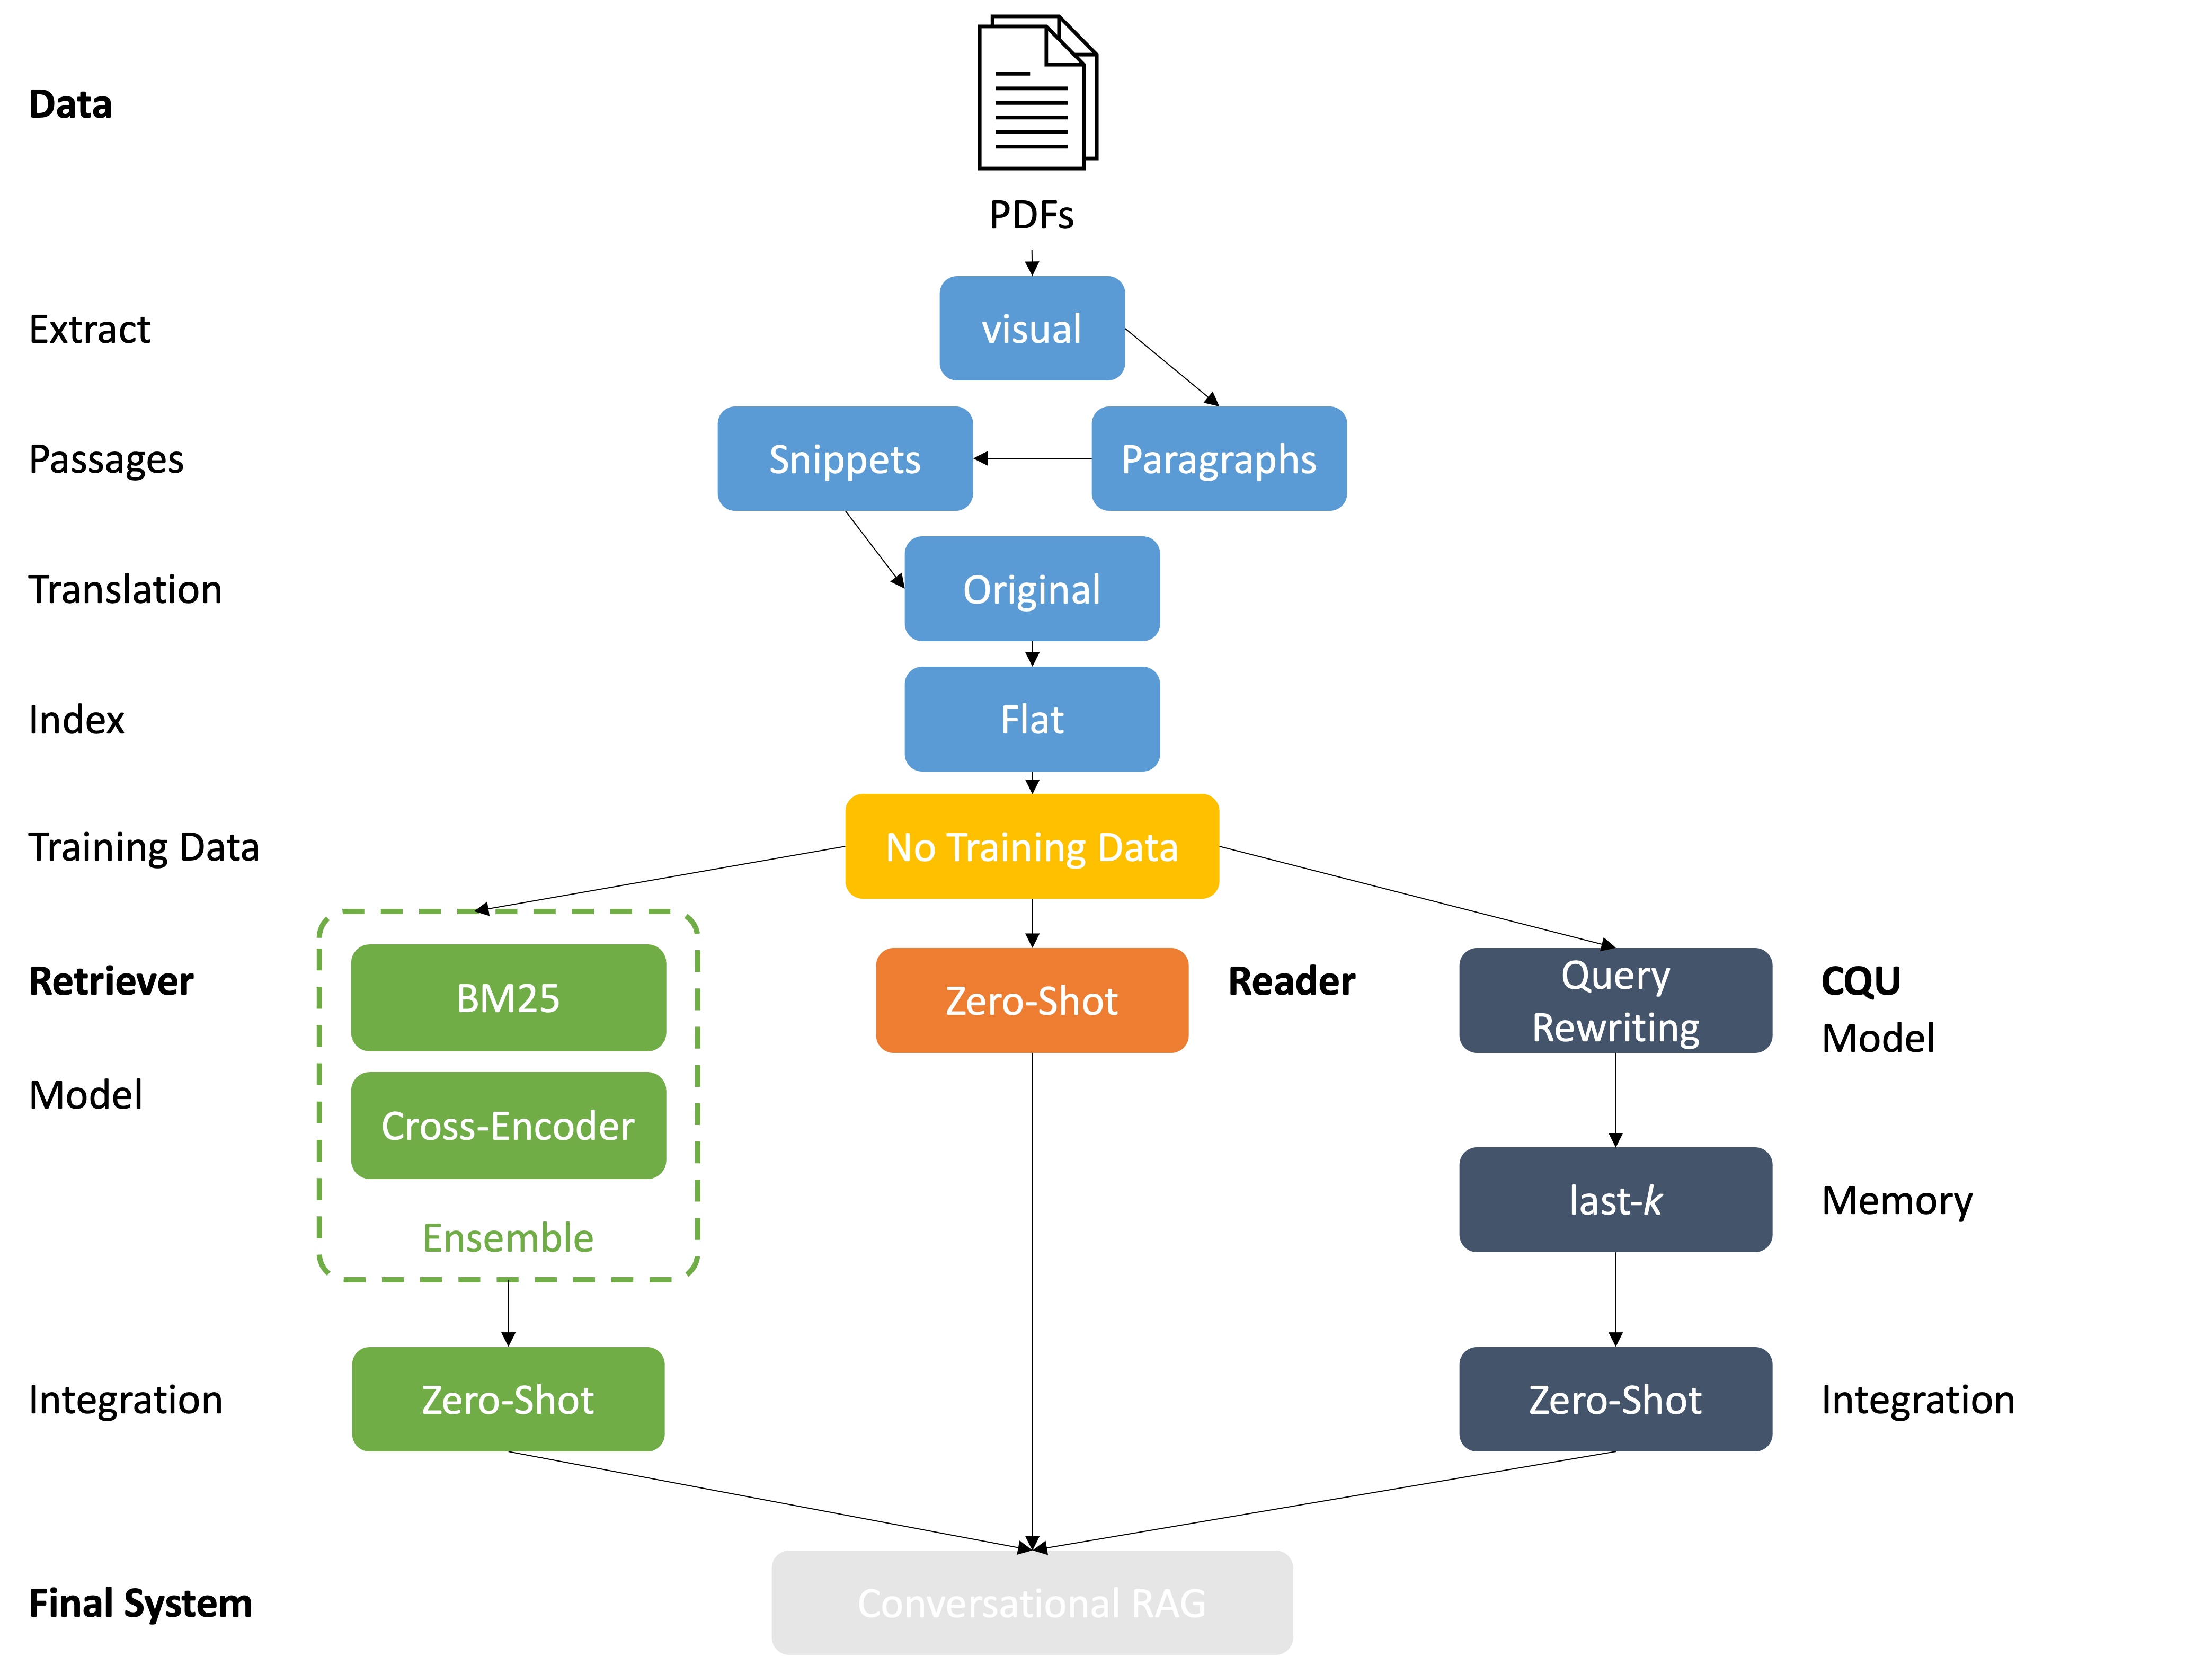
\includegraphics[width=\textwidth]{Grafiken/example_decission_tree.png}
%     \caption{Example of applying the Framework to a System Implementation}
%     \label{fig:example_decission_tree}
% \end{figure}



\subsection{Extract}
\label{subsec:extract}

The sub-task of \textit{Inforamtion Extraction} was defined in the previous section as sub-task (1) of the model $\mathbf{M}$. Given a set of documents $D$, the knowledge source $P$ needs to be extracted using \textit{Information Extraction} techniques in combination with \textit{Passage Extraction} operations. As synthetic data generation is also part of the extraction component according to Section \ref{sec:overview}, it will also be discussed in this section. This is originally not part of the model $\mathbf{M}$, but makes from a system architecture sense, to place these operations in this system component. Synthetic Data can be seen as a separate task, which has nothing to do with the original task of \gls{convqa}, but is a necessary step in order to train components of the model $\mathbf{M}$ or evaluate those.

\vspace{\baselineskip} % Add one line space

\textbf{Information Extraction:} When it comes to extracting text from any document $d$, there are many approaches to choose from. Some extract structures, metadata, or similar, which can be further utilized, while others extract unstructured text only. In any case, this extraction process highly depends on the source document type. An HTML website requires different approaches and tools compared to a PDF, for instance. An example tool for direct extraction of PDFs is Py2PDF \cite{noauthor_welcome_nodate}. Regardless of the source document and tool used to extract textual information $C_d$, there are two major possible outcomes given a set of documents $D$:

\begin{enumerate}
    \item \textit{Structured Extraction:} Denoted as $f_{StrucExt}(\cdot)$, in this extraction operation, $C_d$ can be extracted into logical segments directly: $f_{StrucExt}(d) = \{c_{d_i} \subset C_d : i \in \{1, 2, \ldots, n\}, C_d = \bigcup_{i=1}^{n} c_{d_i}\}$. If $f_{StrucExt}$ is applied to all documents $d$ in $D$, the resulting set $C$ contains all the outputs of $f_{StrucExt}$ for each document in $D$. Formally, $f_{StrucExt}(D) := C = \{C_{d_1}, C_{d_2}, \dots, C_{d_m}\}$, where each document $d$ is transformed into a set of logical segments $C_{d_i}$ representing its content.
    \item \textit{Unstructured Extraction:} Denoted as $f_{UnstExt}(\cdot)$, when applied to $D$, it results in a concatenated text corpus $C_d = \{c_d\} $ containing the textual content of a document $d$: $f_{UnstExt}(D) := C = \{C_{d_1}, C_{d_2}, \dots, C_{d_n}\}$, where each document $d$ is transformed into a single text snippet $c_d$ representing its content.
\end{enumerate}

In order to generate snippets $p$ from $C$, \textit{Passage Extraction} has to be applied on $C$.

\vspace{\baselineskip} % Add one line space

\noindent\textbf{Passage Extraction:} The implementation of passage splitting depends on the nature of $C$ and the desired granularity of the output. In general, there are three operations for constructing passages $p$ based on a text snippet $c_d$:

\begin{enumerate}
    \item \textit{Paragraphs:} $f_p(\cdot)$ is an operation that transforms a collection $C_d$ of texts $c_d$ into a set of passages $P = \{p_1, p_2, \dots, p_n\}$. It operates similarly to $f_{StrucExt}(\cdot)$, but instead of $D$, it operates on $C_d$. The output of $f_p(\cdot)$ consists of passages $p$ that represent logical segments of the text corpus $c_d$. Usually, it operates in a \textit{rule-based} manner, meaning that a paragraph is defined by a token indicating a paragraph (e.g., \textit{<p/>} in HTML). The length $l$ of each $p_i$ is variable, and the number of paragraphs $|P|$ can also vary.
    \item \textit{Snippets:} $f_s(\cdot)$, when you have a fixed passage length $l$, divides the concatenated text $c_d$ into $|c_d|\bmod{l} + 1$ passages $p$ per $c_p$. Alternative approaches may involve specifying minimum and maximum lengths, denoted as $l_{\text{min}}$ and $l_{\text{max}}$. The exact point of division depends on whether a sentence ends within the specified window or not. If a sentence ending is found within the window, the snippet concludes at that point. Otherwise, it concludes at the end of the window. The individual length of the extracted passages $P = \{p_1, p_2, \ldots, p_n\}$ is not fixed in the case of syntactic snippets, as well as the number of paragraphs $|P|$.
    \item \textit{Sliding Windows:} $f_w(\cdot)$ utilizes a window size $l$, a concatenated text $c_d$, and a step size $s$. The window slides over the text $c_d$, and the text within the window is used as a passage $p$. This results in $\frac{|c_d| - l}{s}$ passages, denoted as $P = \{p_1, p_2, \ldots, p_n\}$.
\end{enumerate}

These operations can be combined in a pipeline fashion. For example, first $f_p(C_d) := P_{paragraphs} = \{p_{paragraphs,1}, p_{paragraphs,2}, \dots, p_{paragraphs,n}\}$ is constructed, and afterward, on the logical paragraphs, $f_w(f_p(C_d)) := f_w(P_{paragraph}) = P_{window} = \{p_{window,1}, \allowbreak p_{window,2}, \allowbreak \dots, p_{window,i}\}$ is applied. The way these operations are combined is highly use-case specific and needs to be evaluated for each use-case individually. Another important factor influencing the decision regarding the parameters $l$, in general, the operation used, is the desired model for the \textit{Retriever} and \textit{Reader} as they may be trained on a specific token length as input or have a maximum length of tokens they accept as input or require a certain clarity of data points.


\vspace{\baselineskip} % Add one line space
\noindent\textbf{Synthetic Training Data Generation:} This can be interpreted as a knowledge distillation task. The main idea is to use a model $ED(\cdot)$ to generate a synthetic dataset for the sub-task and problem field of \textit{Passage Retrieval} and \textit{Response Generation}:

\begin{equation}
    ED(P) := (P, Q)
    \label{eq:task}
\end{equation}

Where $P = \{p_1, p_2, \dots, p_n\}$ corresponds to a corpus of passages to retrieve from and $Q$ is a set of questions. If $\mathcal{I}(q,p) = 1$, this means that the passage reflects the question's search intent. Given this task, there are several synthetic dataset types:

\begin{enumerate}
    \item \textit{Questions given Context} $ED_{qp}(p) := q_s$: Given a passage $p$, generate a synthetic question $q_s$ that satisfies the desired search intent. Applying $ED_{qp}(P)$ to a set of passages will generate a set of questions $Q_s = \{q_1, q_2, \dots, q_n\}$, with one question for every passage, i.e., $|Q_s| = |P|$. $ED_{qp}$ can also be applied multiple times with different intents to generate multiple different questions $q_{s,j,1}, q_{s,j,2}, \dots , q_{s,j,i}$ for a single passage $p_j$.
    \item \textit{Question-Context-Answer Triples} $ED_{qpa}(p) := (q_s, p, a_s)$: Given a passage $p$, generate a synthetic question $q_s$ that satisfies the search intent and provides an answer $a_s$, where $\mathcal{I}(q_s, a_s) = 1 \land \mathcal{I}(q_s, p) = 1 \land \mathcal{I}(a_s, p) = 1$. The result of applying $ED_{qpa}(P)$ to a set of passages is a set of question-passage-answer triples $QPA_s = \allowbreak \{(q_{1,s}, p_1, a_{1,s}), \allowbreak (q_{2,s}, p_2, a_{2,s}), \allowbreak \dots, (q_{n,s}, p_n, a_{n,s})\}$, where $|QPA_s| = |P|$. $ED_{qpa}$ can also be applied multiple times with different intents to generate multiple different questions $q_{s,j,1}, \allowbreak q_{s,j,2}, \dots , q_{s,j,i}$ and corresponding answers $a_{s,j,1}, \allowbreak a_{s,j,2}, \dots , a_{s,j,i}$ for a single passage $p_j$.
\end{enumerate}

While the previous two approaches focus on single tuples of either $(q,p)$ or triples of $(q,p,a)$, there is also a problem field of generating conversations based on passages $P = \{p_1, p_2, \dots, p_n\}$ from the same underlying document $d$. Therefore, the task given in Equation \ref{eq:task} is changed to:

\begin{equation}
    ED(P) := (H, P)
    \label{eq:task_conversation}
\end{equation}

Where $H$ corresponds to a set of conversation histories $h$ containing multiple turns. The first turn is always a question $q_1$, followed by an answer $a_1$ based on a passage $p \in P$, also given a search intent $I$ over the whole history $h$. Synthetic datasets for this task can be generated in the following ways:

\begin{enumerate}
    \setcounter{enumi}{2} % Set the starting value to 3
    \item \textit{Conversational Question-Context-Answer Histories} $ED_{cqpa}(E) := H_s$: Given a subset of passages $E \subset P$, the task of the model $ED_{cqpa}$ is it to construct a realistic conversation with an intent over the corpus $E$. The result of applying $ED_{cqpa}(E)$ on a set of passages is a set of conversation histories $H_s = \{h_1, h_2, \dots, h_n\}$. $ED_{cqpa}$ can also be applied multiple times with different intents in order to generate multiple different conversations $h_{s,j,1}, h_{s,j,2} \dots , h_{s,j,i}$ for a single subset of passages $E \subset P$.
\end{enumerate}

There are several ways to implemnt the models $ED_{qp}$, $ED_{qpa}$ or $ED_{cqpa}$. Implementations of those approaches will be discussed in Chapter \ref{chap:eval}. 


% In this pipeline, the prompt-based \gls{qg} method known as PROMPTAGATOR \cite{dai_promptagator_2022} is used to generate a synthetic \gls{qa} dataset for ColBERTv2 \cite{santhanam_colbertv2_2022} based on $P$. The goal is to create triples of $(q, p^{+}, p^{-})$, similar to those found in datasets like MS MACRO \cite{bajaj_ms_2018}. For the task of $E_{qg}(p) := q$, a \gls{s2s} model, specifically a \gls{llm}, will be employed. This technique can be interpreted as knowledge distilation from the LLM to the later trained retriever. Similar to PROMPTAGATOR, there are two approaches to consider:

% \begin{enumerate}
%     \item \textit{Zero-Shot:} In this approach, a single prompt is executed to generate a question $q_i$ corresponding to a passage $p_i$, all without the need for any supervised dataset.
    
%     \item \textit{Few-Shot:} This approach uses $k$ supervised pairs $(q_j, p^{+}_{j})^{k}$ to generate a question $q_i$ corresponding to a passage $p_i \in P$.
% \end{enumerate}

% The prompt used for \textbf{zero-shot \gls{qg}}, where $p_i$ represents a passage from $P$, is:

% \verb|f'{p_i} Read the passage and generate a corresponding query.'|

% The prompt used for \textbf{few-shot \gls{qg}}, where $q_j$ represents a question, $p_j$ the corresponding passage, and $p$ the passage for which a question is being generated, is:

% \verb|f'Passage: {p_1} Question: {q_1} XXX Passage: {p_2} Question: {q_2}|

% \verb|XXX ... XXX Passage: {p} Question:'|

% The result of either of these approaches will be a synthetic training dataset of $(q_s, p^{+})$ tuples. This dataset can be used for fine-tuning the retriever.

% A major issue associated with this form of \textbf{\gls{qg}} is its strict limitation to extractive questions, where the evidence can be derived from a single passage only. This limitation significantly constrains this pipeline. However, it does not necessarily prevent the system from answering more complex questions, such as multi-hop questions. These can be addressed by the \textit{retriever} and \textit{reader} modules.


\subsection{Contextual Query Understanding}
\label{subsec:cqu}

Previously the the model $\mathbf{M}$ for \gls{convqa} was introduced. The \gls{cqu} component is responsible for the \textit{Contextual Query Understanding} task. Essentially, the goal of this task is to identify the necessary information in the history $H$ of a conversation to adapt the expression of the question $q_{i+1}$ into a contextualized question $q_c$, such that $\mathcal{I}(q_c, q_{i+1}) = 1$. This adaptation is crucial, as the \textit{Passage Retrieval} task is executed using a single question $q$ rather than the entire history $H$. Therefore, language challenges may arise between turns, such as pronoun resolution (e.g., it, he, she) or turn references.

\begin{equation}
    CQU(h_{i-k:i}, q_{i+1}) := q_c \mid \mathcal{I}(q_c, q_{i+1}) = 1
\end{equation}

The depth of the history $h_{i-k:i}$ that $CQU$ operates on is a hyperparameter to be chosen. Generally, there are three levels of depth:

\begin{enumerate}
    \item \textbf{K-many:} Consideration of the last $k$ turns.
    \item \textbf{All:} Utilization of the entire history, $k = i - 1$.
    \item \textbf{Memory:} Inclusion of not only the current history but also previous chat histories by this user. The concept of memory will not be further discussed in this thesis, as it opens a whole new field of research and was excluded in the problem statement in Section \ref{sec:overview}.
\end{enumerate}

The decision on depth already implies limitations, as the \textit{K-many} approach may lead to reference errors in a conversation, while too large $k$ increases the computational complexity. This leads to $h_{i-k:i} \subset H$, which is used by the $CQU$.

The \gls{cqu} unit itself can be either an implicit or explicit method. Implicit methods use a one-step approach and are based on the \textit{Transformer} architecture, while explicit methods apply a two-step approach and can vary in implementation:

\begin{equation}
    CQU_{\theta}(h_{i-k:i}, q_{i+1}) := q_c \mid \mathcal{I}(q_c, q_{i+1}) = 1 
    \label{eq:cqu-implicit} 
\end{equation}

Equation \ref{eq:cqu-implicit} shows the transformer-based \gls{cqu} unit with trainable parameters. During the training of the parameters, it is necessary to have an annotated dataset of turns and contextualized questions $q_{c,i}$ for every turn question $q_i$. The loss of the \gls{cqu} will be defined between the human-annotated contextualized question $q_c^*$ and the generated contextualized question $q_c$.

Explicit approaches consist of two operations:

\begin{align}
    rel_{CQU}(x, q_{i+1}) &:= 
    \begin{cases}
        \begin{aligned}
            & x \in C_{q_{i+1}}, & \text{if } x \text{ is relevant for } q_{i+1}\\
            & x \not\in C_{q_{i+1}}, & \text{if }  x \text{ is not relevant for } q_{i+1}
        \end{aligned}
    \end{cases} \\
    rep_{CQU}(C, q_{i+1}) &:= q_c
\end{align}

Where $rel_{CQU}$ is an operation to determine, for a string $x \subset h_{i-k,i}$ (which can be a token, word, or snippet of a turn $h_{i-k,i}$), if it is relevant context to enrich the question $q_{i+1}$. If so, it is added to the context set $C_{q_{i+1}}$. The operation $rep_{CQU}$ works over $C_{q_{i+1}}$ and $q_{i+1}$ to rephrase and generate a contextualized question $q_c$.

The relevance operation can be implemented in multiple ways. Some include \gls{s2s} models or entity matching. The rephrasing operation is a typical \gls{mrc} summary task. Its inputs are the set of context-relevant information $C_{q_{i+1}}$ and the question $q_{i+1}$.

In general \gls{cqu} is an ongoing field of research, especially for follow-up questions and resolving ambiguity. The latest research utilizes more often \gls{llm}s for this task. This thesis won't focus on \gls{cqu}. Please refer to \cite{mao_large_2023} for a state-of-the-art approach.

\subsection{Retriever}
\label{subsec:retriever}

Previously we have divided the main task of a model $\mathbf{M}$ for \gls{convqa} into multiple sub-tasks. The Retriever component handles the \textit{Passage Retrieval} task. The goal of this component is to identify relevant passages $p$ from the knowledge source $P$ given a contextualized question $q_c$. The contextualized question $q_c$ is generated by the \gls{cqu} unit (see Section \ref{subsec:cqu}). Approaches, that are using instead of $q_c$ the whole history $H$ for retrieval, will not be discussed in this thesis. The identification of passages includes a scoring of relevance for each passage $p$ given a question $q_c$. The scoring function $p_{\text{Ret}}(p|q_c)$ is defined as:

\begin{equation}
    p_{\text{Ret}}(p|q_c) = \text{Score}(q_c,p)
    \label{eq:retriever}
\end{equation}

Here, $\text{Score}(q_c,p)$ is a value determining the relevance of a passage $p$ in relation to $q_c$, enabling the ranking of passages $p$ given a question $q_c$. Based on the score, the passages will be ordered in descending order, and the top-$k$ passages will be combined into an evidence set $E_{q_c}$. A different approach is to set a threshold for the $Score(q,p)$ and add all passages $p$ to $E_{q_c}$ for which $Score(q,p)$ surpasses the threshold. Within the evidence set $E_{q_c}$, a passage $p$ will be represented as a tuple $(p, \text{Score}(q_c,p))$. Concerning the evidence set $E_{q_c}$ in relation to the question $q$ and the underlying search intent, the following cases exist:

\begin{equation}
    \forall q \in Q, \exists! E_{q_c} \subset P  := 
    \begin{cases}
        \begin{aligned}
            &1. \text{ } \mathcal{I}(q,E_{q_c} = \emptyset) = 1 \\
            &2. \text{ } \mathcal{I}(q,E_{q_c} = \{p\}) = 1 \\
            &3. \text{ } \mathcal{I}(q,E_{q_c} = \{p_1, p_2, \dots, p_n\}) = 1
        \end{aligned}
    \end{cases}
    \label{eq:evidence_cases}
\end{equation}

For every question, there exists an evidence set. In order for intent $\mathcal{I}(q,E_{q_c})$ to be 1, there are three cases: either the evidence set $E_{q_c}$ has to be empty, $E_{q_c}$ has to have exactly one element $p$, or $E_{q_c}$ has to have multiple passages $p$. To put it more simply, for a given question, the answer is determined either by the evidence that there is no supporting passage $p$, or that there is exactly one passage $p$ containing the requested information, or that multiple passages $p$ contain the necessary information to answer the question $q$.

\vspace{\baselineskip}

\textbf{Retriever}: Depending on the chosen method for a Retriever, the Retriever component can either be trainable or have adjustable parameters:

\begin{align}
    r_{\text{Ret}, \theta} &= \text{Retriever}_\theta(q_c, P) \\
    r_{\text{Ret}, \Theta} &= \text{Retriever}_\Theta(q_c, P)
\end{align}

Here, $\theta$ is the set of trainable parameters, and $\Theta$ is a set of adjustable parameters. Examples of the first type of retriever include dense retrievers like \textit{\gls{dpr}}, as introduced in Section \ref{subsec:qa_retrieval}. Examples of the second type of retriever include sparse retrievers like \textit{BM25}, also introduced in the same section. Regardless of the type of retriever, the operation from Equation \ref{eq:retriever} is applied to each passage $p \in P$, and the top-$k$ passages are selected to form the evidence set $E_{q_c}$. As outlined in Equation \ref{eq:evidence_cases}, some questions may require no evidence to fulfill the search intent. However, with the proposed Retrievers, this is not possible. A retriever $r_{\text{Ret}}$ will always assign a $Score(q,p)$ to every passage given a question and its search intent. Filters are applied to filter out passages with a low score, but this is not part of the retriever itself. The evaluation of the evidence with respect to the search intent and correctly identifying the case at hand will be handled by the Reader component (see Section \ref{subsec:reader}).

\vspace{\baselineskip}

\textbf{Mixture-of-Experts}: To enhance the quality of the evidence set $E_{q_c}$, state-of-the-art research and related work have emphasized the effectiveness of combining multiple retrievers (see Section \ref{sec:related_work}). This combination can be achieved in various ways, which can also be combined further:

\begin{itemize}
    \item \textbf{Re-Ranking}: This involves the combination of multiple retrievers in a pipeline fashion. In most cases, a fast but imprecise Retriever is used to retrieve a large evidence set, e.g., $r_{BM25}(q_c,P) = E_{q_c,1}$, where $|E_{q_c,1}| = 100$. Subsequently, a second, more accurate Retriever is employed to re-rank the evidence set $E_{q_c}$, e.g., $r_{CE}(q_c,E_{q_c,1}) = E_{q_c,2}$, where $|E_{q_c,2}| = 25$.
    
    \item \textbf{Ensemble}: This idea involves combining multiple retrievers into a single retriever. This can be accomplished by either concatenating the evidence sets $E_{q_c,j}$ or by aggregating the scores of the individual retrievers $r_j$ into a single score. Formally:
    
    \begin{align}
        \forall r \in R: E_{q_c} &= \bigcup_{j=1}^{|R|} r_j(q_c, P) \\
        \forall p \in P: \text{Score}(q_c, p) &= f(r_1(q_c, p), r_2(q_c, p), \dots, r_{|R|}(q_c, p))
    \end{align}
    
    Here, $f(\cdot)$ represents a function that combines the scores of the individual retrievers $r_j$, for example, using $max(\cdot)$. $R$ is a set of retrievers $r$.
    
    \item \textbf{Weighting}: This approach involves running two retrievers in parallel and multiplying their scores for each passage $p$. It can be seen as a sub-case of ensemble. Formally:
    
    \begin{equation}
        \forall p \in P: \text{Score}(q_c, p) = \prod_{j=1}^{|R|} \alpha_j \cdot r_j(q_c, p), \sum_{j=1}^{|R|} \alpha_j = 1
    \end{equation}
    
    Here, $R$ represents a set of retrievers $r_j$, and $\alpha_j$ is the weight assigned to each retriever $r_j$. These weights $\alpha_j$ can be either fixed or trainable.
\end{itemize}

\vspace{\baselineskip}

\textbf{Fine-Tuning:} A potential issue that may arise for a retriever and a knowledge base $P$ is the misalignment between the underlying formats of the passages $p$ and the formats on which the retriever $r_{Ret,\theta}$ was trained. To address this discrepancy, fine-tuning can be employed to adjust the retriever based on the specific formats used in the given use case.

Given a dataset of tuples $(q, p)$, as described in Section \ref{subsec:extract}, a retriever with trainable parameters $r_{\text{Ret}, \theta}$ can undergo fine-tuning. The first step involves creating the training data $\mathcal{TD} = \{\langle q_i, p_i^+, p_{i,1}^-, \dots, p_{i,n}^-\rangle\}_{i=1}^m$. In this dataset, we already have tuples that contain a question $q_i$ and a positive passage $p_i^+$. The primary objective is to sample $n$ negative passages $p_{i,j}^-$ for each positive passage $p_i^+$. Various methods can be employed \cite{karpukhin_dense_2020}:

\begin{enumerate}
    \item Randomly sampling passages from the knowledge source $P$, where $p_{i,j}^- \in P$ and $p_{i,j}^- \neq p_i^+$.
    \item Retrieving evidence passages using a high-performing \gls{ood} retriever $r_{\text{Ret},\text{OOD}}$ and sampling from the evidence set $p_{i,j}^- \in E_{q_i}$, ensuring $p_{i,j}^- \neq p_i^+$.
    \item Sampling passages from other tuples $(q_k,p_k)$ in the dataset, where $p_k \neq p_i^+$.
\end{enumerate}

Method (1) is the simplest but does not yield high-quality negative passages $p_{i,j}^-$. Method (2), while more complex, typically provides a higher-quality evidence set $E_{q_i}$ than method (1). Method (3) can also be applied in-batch, known as \textit{in-batch negatives}, during the training process. This means that given a batch $B$ of $|B|$-many $(q_i,p_i^+)$ tuples, the negative passages $p_{i,j}^-$ are derived from the positive passages of the other tuples in the same batch $B$. Consequently, this results in $|B| \times |B| - 1$ negative passages $p_{i,j}^-$ per batch $B$ per question $q_i$.

After the construction of the training dataset $\mathcal{TD}$, the retriever $r_{\text{Ret}, \theta}$ can be trained straightforwardly. The forward pass is simply the score prediction of the retriever for every passage, positive and negative, within a tuple of the $\mathcal{TD}$. Therefore the loss function can be defined as follows:

\begin{equation}
    \mathcal{L}(q_i, p_i^+,p_{i,1}^-, \dots, p_{i,n}^-) = -\log \frac{e^{\text{Score}(q_i,p_i^+)}}{e^{\text{Score}(q_i,p_i^+)} + \sum_{j=1}^{n} e^{\text{Score}(q_i,p_{i,j}^-)}}
\end{equation}

The calculated loss will be used in backpropagation to update $\theta$.

The process of fine-tuning needs adaptation when using \textit{synthetically generated data} due to the potential quality issues of the synthetic dataset. To address this, the dataset must be iteratively filtered during the training process. Given a synthetic dataset $\mathcal{TD_s} = \{\langle q_i, p_i^+\rangle\}_{i=1}^m$, a retriever $r_{\text{Ret}, \theta}$ with trainable parameters $\theta$, and a high-performing out-of-domain (\gls{ood}) retriever $r_{\text{Ret},\text{OOD}}$, the following procedure is based on the proposed approach of PROMPTAGATOR \cite{dai_promptagator_2022}:

\begin{enumerate}
    \item Extend $\mathcal{TD_s}$ by adding $n$ negative passages $p_i^-$ for every tuple using Method (2) from above with $r_{\text{Ret},\text{OOD}}$.
    \item Train $r_{\text{Ret}, \theta}$ for $s$ iterations on $\mathcal{TD_s}$ while applying in-batch negatives, as described in Method (3) above.
    \item Filter $\mathcal{TD_s}$ using $r_{\text{Ret}, \theta}$ and $r_{\text{Ret}, \text{OOD}}$ by removing all tuples $(q_i, p_i^+)$ where $p_i^+$ is not in the Evidence set $E_i$, given a parameter $k$, for either $r_{\text{Ret}, \theta}$ or $r_{\text{Ret}, \text{OOD}}$.
\end{enumerate}

Figure \ref{fig:retriever-fine-tuning} illustrates the fine-tuning process with synthetic data. Steps (2) and (3) are repeated cyclically, with step (3) concluding each cycle. After $s$ epochs, $\mathcal{TD_s}$ is filtered once, retrained for $s$ epochs, refiltered, and finally trained again for $s$ epochs. This process may appear counterintuitive, as the retriever is trained on the dataset it's supposed to filter. However, experiments from related work \cite{dai_promptagator_2022} have demonstrated that this approach still yields favorable results. 

Alternative approaches to filtering synthetic datasets may rely solely on high-performing $r_{\text{Ret}, OOD}$. For a synthetic question $q_s$, the evidence set $E_{q_s}$ is generated using $r_{\text{Ret}, OOD}$ with high values for $k$. If $E_{q_s} = \emptyset$, the tuple $(q_s, p_s^+)$ is excluded from $\mathcal{TD_s}$. This approach is simpler but may result in a performance loss. It can be improved by incorporating multiple different high-performing $r_{\text{Ret}, OOD}$ and combining via union their evidence sets $E_{q_s}$.


\begin{figure}[H]
   \centering
    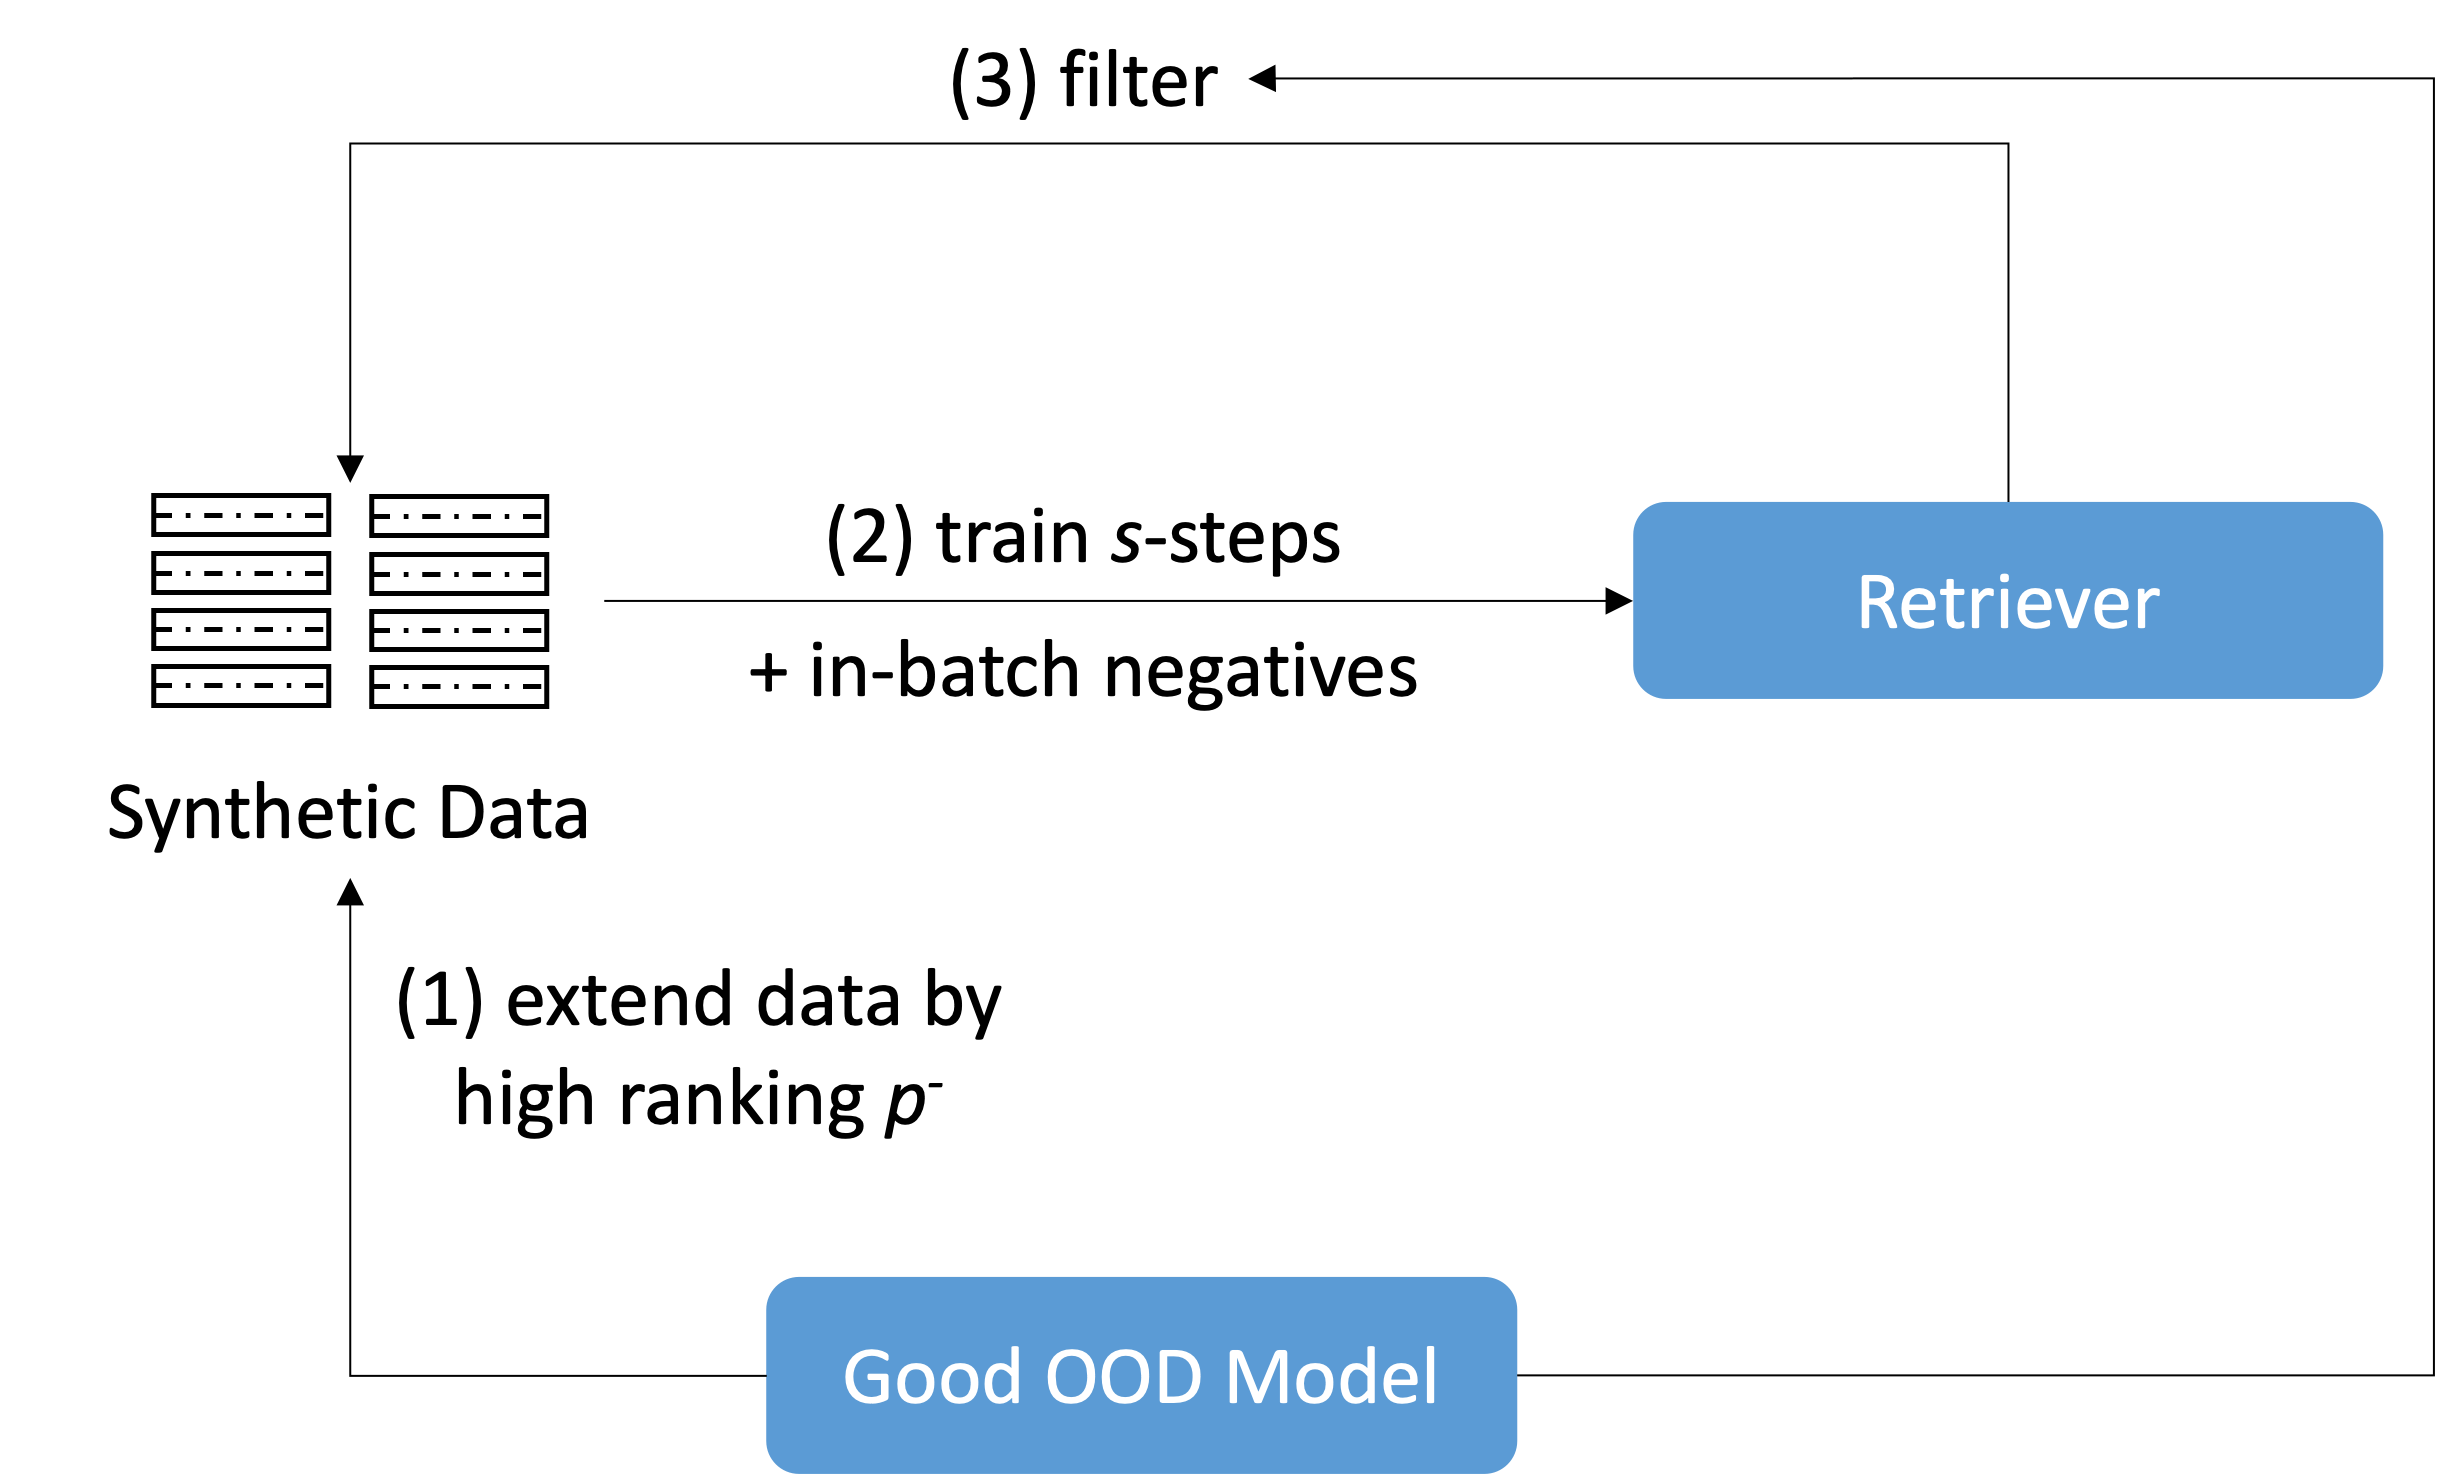
\includegraphics[width=0.8\textwidth]{Grafiken/Training.png}
    \caption{Fine-Tuning Process for Retriever}
    \label{fig:retriever-fine-tuning} 
\end{figure}

\vspace{\baselineskip}

\textbf{Metadata-Filtering:} In certain search scenarios, it may be necessary to filter the knowledge source $P$ by metadata. State-of-the-art open-domain datasets and benchmarks usually don't develop solutions for this problem. However, in real-world scenarios, this is a common user desire.

A filtering request can be understood as the already established intent-fulfilling retrieval task performed over $P$, extended by a consideration of the metadata $M_d$ of the documents $d \in D$ from which $p$ originates. As established in Definition \ref{def:passage_model}, $p = (content, UID_p, UID_d)$ and $d = (C_d, M_d, UID_d)$. Therefore, $\forall p \in P: \exists! M_d$ such that $M_p = M_d$. The task of filtering can therefore be understood as follows:

\begin{equation}
    m_{\text{Ret}}(p|q_c) =
    \begin{cases}
        p \in E_m, & \bigcap\limits_{i=p_1}^{\substack{E_{q_c}}} M_{i} \subset M_p \\
        p \notin E_m, & \bigcap\limits_{i=p_1}^{\substack{E_{q_c}}} M_{i} \not\subset M_p
    \end{cases}
\end{equation}

Here, a passage $p$ is only added to the evidence set $E_m$ if the intersection of all metadata of the passages, in the perfect intention-fulfilling evidence set $E_{q_c}$ of a question $q_c$, is a subset of the metadata $M_p$ of the passage $p$.

In the retrieval process itself, the two tasks of metadata-filtering ($m_{\text{Ret}}$) and scoring ($p_{\text{Ret}}$) can be executed sequentially or combined. This depends on the implementation of the actual index. Some approaches towards metadata-filtering in \gls{convqa} are the following:

\begin{enumerate}
    \item \textbf{Metadata Passage Integration:} In this approach, the metadata $M_p$ is integrated into the \textit{content} of a passage $p$. This enables a one-step approach to retrieval. The retriever will perform scoring and metadata filtering simultaneously. However, in this approach, the original form of the metadata $M_p$, a collection of key-value pairs, will not be utilized. Instead, the metadata will be added implicitly (e.g., embedding addition) or explicitly (e.g., attaching keywords) to the \textit{content} of $p$, leading to a loss in the functionality of the metadata, which could cause issues like a not fully applied filtering.
    \item \textbf{Separate Metadata Index:} In this approach, two indices are created and utilized, one representing the passages' \textit{content} and the other representing the passages' metadata. During retrieval, the retriever follows a two-step approach. Ideally, the metadata-filtering task is executed first, and then the scoring task is performed on $E_m$: $E_{q_c} = p_{\text{Ret}}(m_{\text{Ret}}(q_c,P))$.
    \item \textbf{Hierarchical Index:} The hierarchical index utilizes a scoring function $p_{\text{Ret}}$ as the metadata filter. In this approach, in addition to the passage index, a secondary metadata index is employed, typically representing the set of documents $D$. Instead of using $M_d$ as key-value pairs, a document $d$ is encoded in this index as \textit{content}, resembling a passage $p$. This \textit{content} may include a document summary, a concatenation of metadata keywords, or similar information. During retrieval, the retriever initially generates an evidence set $E_m$ by executing $p_{\text{Ret}}(q_c, D)$, followed by the execution of $p_{\text{Ret}}(q_c, E_m)$ to form the ultimate evidence set $E_{q_c}$: $E_{q_c} = p_{\text{Ret}}(p_{\text{Ret}}(q_c, D))$. This approach carries the same issues as (1) but is useful when the metadata $M_d$ are not simple entity or number-based values, but rather more complex information like a document summary.
\end{enumerate}

\subsection{Reader}
\label{subsec:reader}

The Reader component handles the \textit{Response Generation} task. The goal of this component is to extract an answer $a$ based on the evidence set $E_{q_c}$ given a question $q$. The answer $a$ can be a single token, a span of tokens, or a set of tokens. The answer extraction can be defined as follows: $r_{\text{Read}}(E_{q_c}, q) := a$. Depending on the desired utility of the Reader, the Reader can also incorporate \textit{Context Query Understanding} capabilities and therefore receive, in addition to the evidence set $E_{q_c}$ and question $q$, the history $H$ as input. This leads to the following two variations:

\begin{align}
    r_{\text{1-Reader}}(E_{q_c}, q_c) &:= a \label{eq:reader} \\
    r_{\text{k-Reader}}(E_{q_{i,c}}, q_{i}, H) &:= a_{i} \label{eq:reader_context}
\end{align}

Enhancing the theoretical model $\mathbf{M}$ from Definition \ref{def:task} with the system requirements defined in Section \ref{sec:overview}, the challenges for the Reader component can be broken down into the following:

\begin{enumerate}
    \item Generate an answer $a$ based on the evidence set $E_{q_c}$ that satisfies the search intent $\mathcal{I}(q_c, a) = 1$.
    \item As stated in Equation \ref{eq:evidence_cases}, there are three cases for the evidence set $E_{q_c}$ in relation to the question $q$ and the underlying search intent. The Reader component has to identify the case at hand and determine the final gold-evidence set $\hat{E}_{q_c} \subset E_{q_c}, \quad \mathcal{I}(q_c, \hat{E}_{q_c}) = 1$.
    \item Identify ambiguity in questions $q_{i}$ and determine a corresponding clarification question $a_{i}$ which steers the user towards a more specific question in the next turn $i+1$.
    \item Chatlike behaviour is expected for \gls{convqa}. This may include the ability of \textit{Contextual Query Understanding}, but also challenges like (3). In general, this challenge describes the model's capability to generate a human-like conversation. 
\end{enumerate}

At the core of the Reader's implementation is the evidence set $E_{q_c}$. It is constructed using the methods outlined in Section \ref{subsec:extract}. However, it hasn't been discussed yet what exactly is a good format for a passage $p$ in the evidence set $E_{q_c}$ for the Reader. Basically, all variations of the passages $p$ can be broken down to the following scale:

\begin{figure}[H]
    \centering
    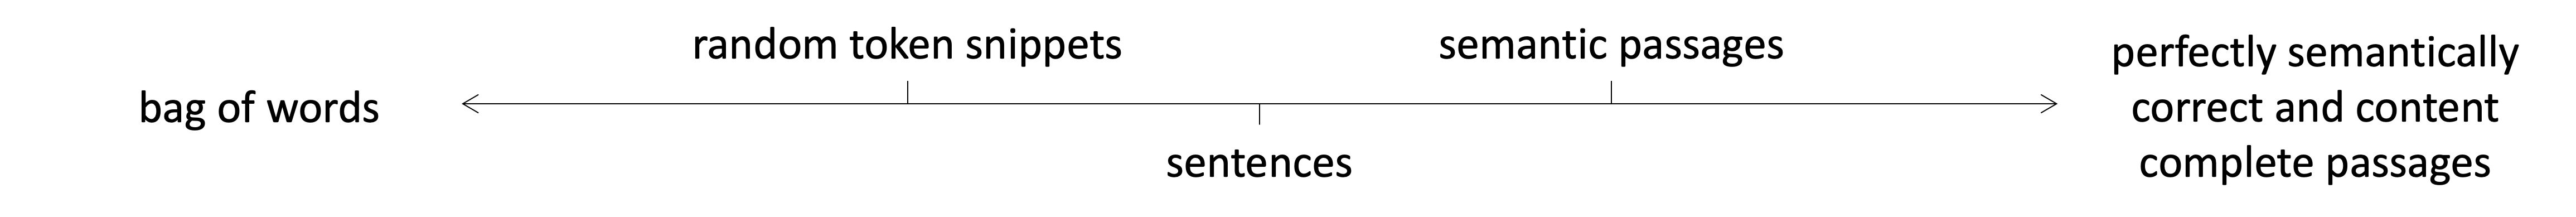
\includegraphics[width=1\textwidth]{Grafiken/Scale_Passages.png}
    \caption{Scale of Passage implementations}
    \label{fig:scale-passages-implementation}
\end{figure}

Most datasets used for \gls{qa}, \gls{convqa}, or training of \gls{prlm} find themselves on the right end of this scale. So, the \gls{llm}s get trained on semantically correct and most of the time content-complete passages $p$. Exceptions are datasets for multi-hop \gls{qa} where the passages are not content-complete, but the aggregation of multiple passages is needed. This evokes the question of how to construct the passages, keeping in mind how the used \textit{Transformer} models have been trained. However, this thesis will not further evaluate the influence of different passage extraction variations, as there is currently no comprehensive research on this topic to the best of our knowledge.

The first challenge (1) of the Reader is closely related to the task \gls{mrc} and classical \gls{qa}. Let's assume that the evidence set is the perfect evidence set that it takes to answer question $q_c$: $E_{q_c} = \hat{E}_{q_c}$. The model from Equation \ref{eq:reader} can be easily trained with a supervised dataset. To fulfill this task, a dataset consisting of question-context-answer triples is necessary, where the context corresponds to $\hat{E}_{q_c}$ and therefore is a list of passages. Depending on the dataset, the model can even be trained to fulfill multiple question types. This can be achieved by varying the question types of the questions in the triples.

The second challenge (2) is more complicated, as in a modular implementation, the Retriever will always pass an evidence set $E_{q_c}$ with a fixed length $|E_{q_c}| = k$ to the Reader. The Reader, therefore, has to incorporate its own mechanism of passage identification. This naturally leads to a trade-off that has to be made. Setting a small $k$-value for the Retriever may reduce the \gls{hr}, and therefore the correct passages won't necessarily be included in the evidence set $E_{q_c}$. On the other hand, the Reader can't handle an arbitrary number of passages, due to the nature of the underlying \textit{Transformer} models. Solutions to this problem may include:

\begin{itemize}
    \item \textbf{Re-Ranker:} The idea of Re-Rankers was already introduced in Section \ref{subsec:retriever}. Basically, before handing $E_{q_c}$ to the Reader, the evidence set is re-ranked by a second Retriever. This second Retriever can be a simple filter over the scores of the passages or an even more complex model than the first Retriever.
    \item \textbf{Compression:} A compressor can iterate over a larger set $E_{q_c}$ than the Reader itself, as it only operates on one passage at a time. The goal of the compressor is to identify the most relevant information of a passage $p \in E_{q_c}$ given the question $q_c$. This compressed information will then create the new evidence set $E_{q_c}$. This approach reduces the number of tokens the evidence set $E_{q_c}$ consists of and therefore enables larger $k$-values for the Retriever. It is similar to a Re-Ranker.
    \item \textbf{Multi-Retrieval:} The concept of Multi-Retrieval involves triggering multiple retrievals until a certain level of satisfaction is reached regarding the evidence set $E_{q_c}$. The specific approaches may vary and will not be further discussed in this thesis.
    \item \textbf{Trained Reader:} The core of this idea is to train a Reader on a dataset consisting of question-context-answer triples, where the context is a list of passages, which not necessarily is the gold-evidence set $E_{q_c} \not= \hat{E}_{q_c}$. The Reader will learn to identify the correct passages and therefore can be used to filter the evidence set $E_{q_c}$ himself. 
    \item \textbf{Parametric Knowledge:} This approach is the fundamental idea of \gls{rag}. The underlying \textit{Transformer} of the Reader gets trained on the knowledge source $P$ to store implicitly the knowledge. This may lead to a better understanding of the evidence set $E_{q_c}$ and give the Reader the ability to access knowledge, which is not included in $E_{q_c}$ (e.g., when $\hat{p} \not\in E_{q_c}$). The fine-tuning itself is the common adoption of a \gls{prlm} to a small new knowledge source $P$. During fine-tuning the \gls{prlm} is tasked to predict the next token and therefore learn the knowledge source $P$ specific language and knowledge.
\end{itemize}

Given the (3) challenge, the Reader must be able to determine ambiguous questions $q_{i}$ and generate a clarification question $a_i$. This task consists of two steps:

\begin{enumerate}
    \item \textbf{Identify Ambiguity:} Given a question $q_i$, the Reader $r_{\text{Read}}(\cdot)$ has to determine if the question $q_i$ is ambiguous. A question is ambiguous if there are multiple answers that fulfill the question's search intent, but themselves satisfy different intents ($\mathcal{I}(q_{i}, a_{i,1}) = 1 \quad \allowbreak \land \quad \allowbreak \mathcal{I}(q_{i}, a_{i,2}) = 1 \quad \allowbreak \land \quad \allowbreak \mathcal{I}(a_{i,1},a_{i,2}) = 0$). The ambiguity in $q_i$ can either originate in a factoid ambiguity (e.g., $\mathcal{I}(q_{i}, p_1) = 1 \quad \land \quad \mathcal{I}(q_{i}, p_2) = 1 \quad \land \quad \mathcal{I}(p_1, p_2) = 0$) or a linguistic ambiguity (e.g., ambiguous cross-references).
    \item \textbf{Resolve Ambiguity:} Given an ambiguous question $q_i$, the Reader $r_{\text{Read}}(\cdot)$ has to generate a clarification question $a_i$ that resolves the ambiguity via the user's next question $q_{i+1}$. Meaning that $\exists! a_{i+1} : \mathcal{I}(q_{c,i+1}, a_{i+1}) = 1$.
\end{enumerate}

As can be observed, \textit{Clarification Questions} can only be generated and resolved in a dialog and not in a single-turn \gls{qa} scenario. Therefore, it is necessary to train a Reader on a conversational dataset. The dataset is a history $H$, providing for every turn a quadruple of the question-contexts-answer-ambiguity flag. The answer is an annotated clarification question in case of a positive ambiguity flag. Therefore, the \textit{Transformer} model can be trained to identify ambiguity in a question given context and generate a clarification question.

This history-based dataset leads to the challenge (4) of a Reader in this thesis context. Challenge (4) is a more abstract requirement for the reader. It requires the language and generated text to linguistically mimic the language and behavior humans would use in a conversation. In order to fine-tune a \textit{Transformer} model to be able to perform text generation which is more human conversation-like, a dataset of human conversation histories $H$ is needed. This involves a diverse set of training and fine-tuning strategies, which will not be discussed in this thesis. As a reference for this topic, the reader is referred to the work of Touvron et al. \cite{touvron_llama_2023}.

As observed, the Reader's ability to address challenges (1-4) is highly dependent on the training datasets and fine-tuning methods. The challenges defined in this thesis do not cover every possible requirement that someone might have for their \gls{convqa} system. Naturally, larger and more capable models exhibit higher zero- and few-shot performance. Previous solutions mainly focused on fine-tuning \gls{llm}s to address challenges in the Reader (e.g., Noise in the Evidence Set or Negative Rejection). However, as this thesis aims to provide a solution for resource-constrained systems (see Section \ref{sec:overview}, Objective 5 of the \gls{qa} system), the following approach will be presented based on simplifying the overall task of a Reader to address these challenges without fine-tuning.

\vspace{\baselineskip}

\textbf{Chain-, Chain-of-Thought- and Agent-Reader:} Drawing inspiration from the work of Langchain \cite{noauthor_langchain-ailangchain_nodate}, Wei et al. \cite{wei_chain--thought_2023} and Kuhn et al. \cite{kuhn_clam_2023}, the diverse task of a Reader can be broken down into a sequential decision-based procedure. The core idea is to break down the multiple challenges a Reader has to solve into smaller tasks that are easier to solve independently. An easy implementation could involve breaking down the holistic task of the reader into simple sub-tasks that follow a sequential order. One sub-task is for example: \textit{Is the question ambiguous?}. The Reader will be prompted to solve this sub-task, and depending on the result, other sub-tasks will be triggered. This is a rigid activity diagram-like implementation and is similar to the concept of \textit{Chains} in \textit{Langchain}. This can be further improved by adding more flexibility, where the Reader is fine-tuned in a \textit{\gls{cot}} manner to reason over a question, given the evidence and the history. The single challenges or sub-tasks can, therefore, be interpreted as reasoning steps. This requires a whole new dataset for fine-tuning. Extending this idea further, the Reader is developed into an agent, similar to the \textit{ReAct} approach, where it can reason over a question given the evidence and the history, and also has the ability to take certain actions, such as retrieving more evidence or re-running retrieval with a variation of the contextualized question. These are just some ideas on how the Reader is further extended to increase the quality of the \gls{qa} system. However, this thesis will not further evaluate this idea, as it is not the main focus.

\section{Summary Contribution}
\label{sec:conclusion_contribution}

The main contribution of this thesis is a holistic framework covering the entire \gls{convqa} system, from a collection of documents to detailed approaches used for specific components. To the best of our knowledge, no related work has yet provided such a comprehensive perspective on the problem field of \gls{convqa}.

An often overlooked aspect in related research work is the step of \textit{Extraction}. This is due to the fact that most research work is based on already existing datasets. However, in real-world scenarios, the extraction of passages from documents is a crucial step. This thesis breaks down the extraction into simple operations that can be combined to form an extraction pipeline. The parameters of the pipeline can be adjusted to determine the final passage model.

The thesis does not elaborate on new approaches/algorithms to retrievers itself but rather identifies the problems and tasks the retriever component has in a \gls{convqa} system. Given a retriever and a knowledge base, problems can arise from the retriever towards the data (e.g., misalignment between the underlying formats of the passages and the formats on which the retriever was trained). Therefore, the thesis introduces a fine-tuning method based on generated data using a \gls{llm} and multiple state-of-the-art optimizations. Other problems can arise from the retriever towards the evidence set, namely that the evidence set's quality is not sufficient. In order to address this, the thesis elaborates on the concept of \textit{Mixture-of-Experts} as it is an approach that can be used to enhance the retrieval quality without the need to reinvent a new retriever.

Lastly, this thesis introduces the approach of breaking down the task of a reader into challenges. These challenges can be of any nature (e.g., identifying ambiguity in questions or assessing the completeness of the evidence set). Previous related work has not yet broken down the challenges towards a reader in such a manner to the best of our knowledge. Given these small and well-defined challenges, it's easy to identify possible solutions regarding the reader. In this thesis, multiple such solutions based on related work are introduced, and new ones for specific challenges are proposed, mainly focusing on fine-tuning. On top of that, the thesis introduces the idea of using these smaller, finite, and simpler challenges of the whole reader task to create a sequential decision-based procedure, which could enable smaller \gls{llm}s to solve the reader task without performance losses compared to larger \gls{llm}s.


% \section{Question Answering over PDFs}
% \label{sec:qa-over-pdfs}

% \begin{figure}
%     \centering
%     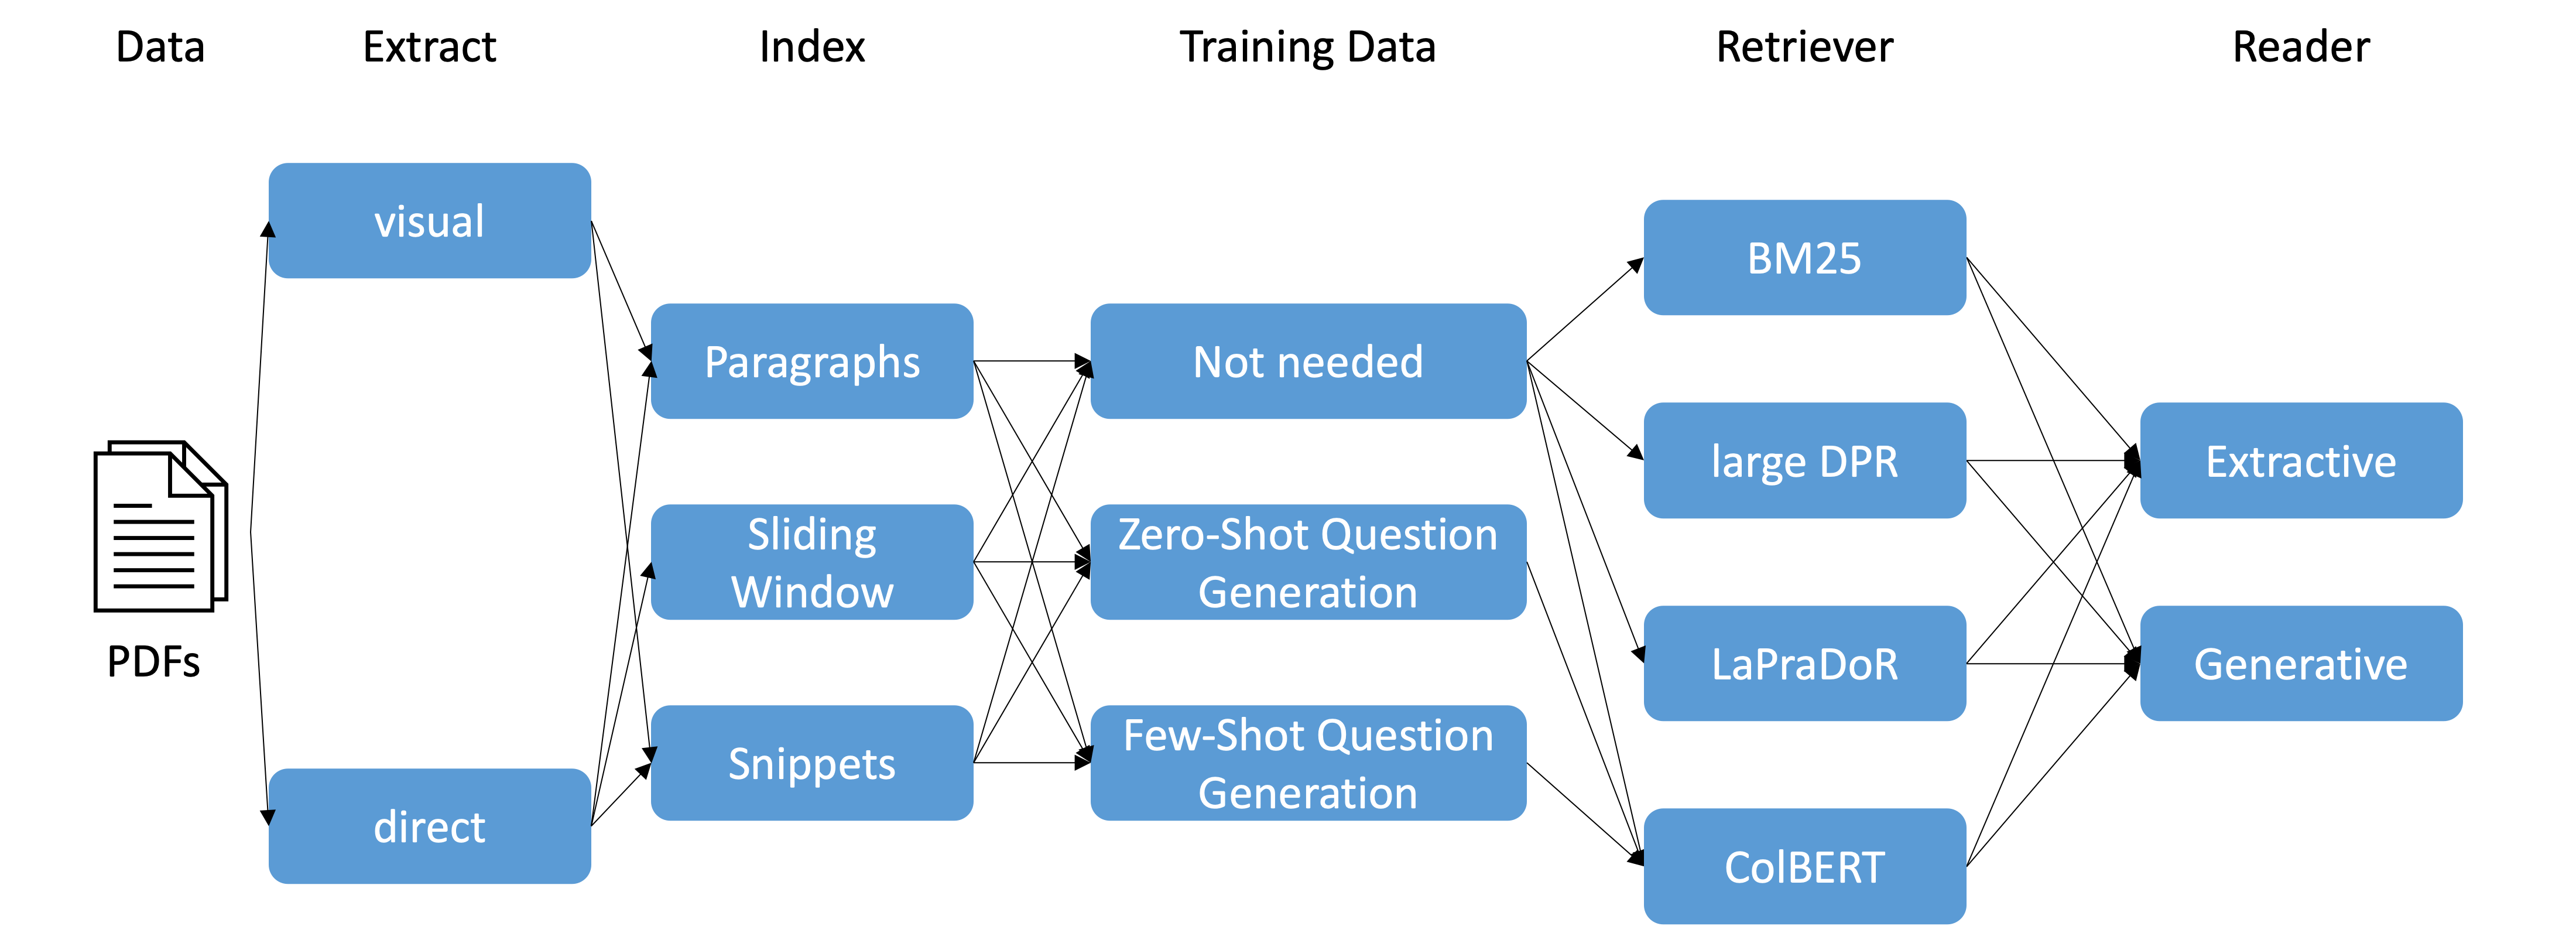
\includegraphics[width=0.8\textwidth]{Grafiken/Possible_Systems.png}
%     \caption{Possible Combinations of Modules to Create an Adapted QA-System}
%     \label{fig:qa-system-combinations}
% \end{figure}

% The possible combinations of modules to create an adapted \gls{qa}-System can be seen in Figure \ref{fig:qa-system-combinations}.


% \subsection{Extract}
% \label{subsec:extract}
% %%%%%

% \subsection{Retrieve}
% \label{subsec:retrieve}

% \textbf{Out-of-Domain Retrievers:} The easiest implementation is the out-of-domain usage of retrievers without fine-tuning and the need for generating a training dataset. Three major retrievers seem promising due to their performance on the BEIR \cite{thakur_beir_2021} out-of-domain benchmark for retrievers:

% \begin{enumerate}
%     \item \textit{BM25} is the standard Sparse Retriever based on lexical probabilistic matching between the query $q$ and passages $p$.
%     \item \textit{Large DPRs} are Dense Retrievers based on large encoders. They utilize typical dense retrieval paradigms and are a primary approach in open-source projects like \textit{Langchain} \cite{noauthor_langchain-ailangchain_nodate}.
%     \item \textit{LaPraDoR} is a hybrid retriever based on a broadly trained Representation-based Retriever, similar to (2), combined with lexical weighting (1).
% \end{enumerate}

% The \gls{laprador} utilizes the advantages of both lexical and semantic search. Given a question $q$ and a passage $p$, the semantic similarity $\text{sim}(q,d)$ is calculated using a \gls{dpr} model. In addition, the lexical similarity $\text{BM25}(q,d)$ is calculated. The final score $\text{score}(q,d)$ is computed as follows:

% \begin{equation}
%     \mathbf{score}(q, d) = \mathbf{sim}(q, d) \cdot \mathbf{BM25}(q, d)
% \end{equation}

% This approach achieves state-of-the-art performance on the BEIR benchmark without the need for fine-tuning. It serves as the ideal off-the-shelf component for the desired \gls{qa}-System.

% \noindent\textbf{Fine-Tuning Retrievers:} Fine-tuning is a challenging task in the absence of a supervised dataset, especially when dealing with a Representation-Interaction Retriever like ColBERTv2. Currently, there is no clear reference on how to fine-tune a Representation-Interaction Retriever like ColBERTv2 on synthetic data. To address this gap, this thesis proposes the approach depicted in Figure \ref{fig:retriever-fine-tuning}, which combines elements from the training processes of PROMPTAGATOR \cite{dai_promptagator_2022}, the original \gls{dpr} \cite{karpukhin_dense_2020}, and ColBERTv2 \cite{santhanam_colbertv2_2022}.

% \begin{figure}
%    \centering
%     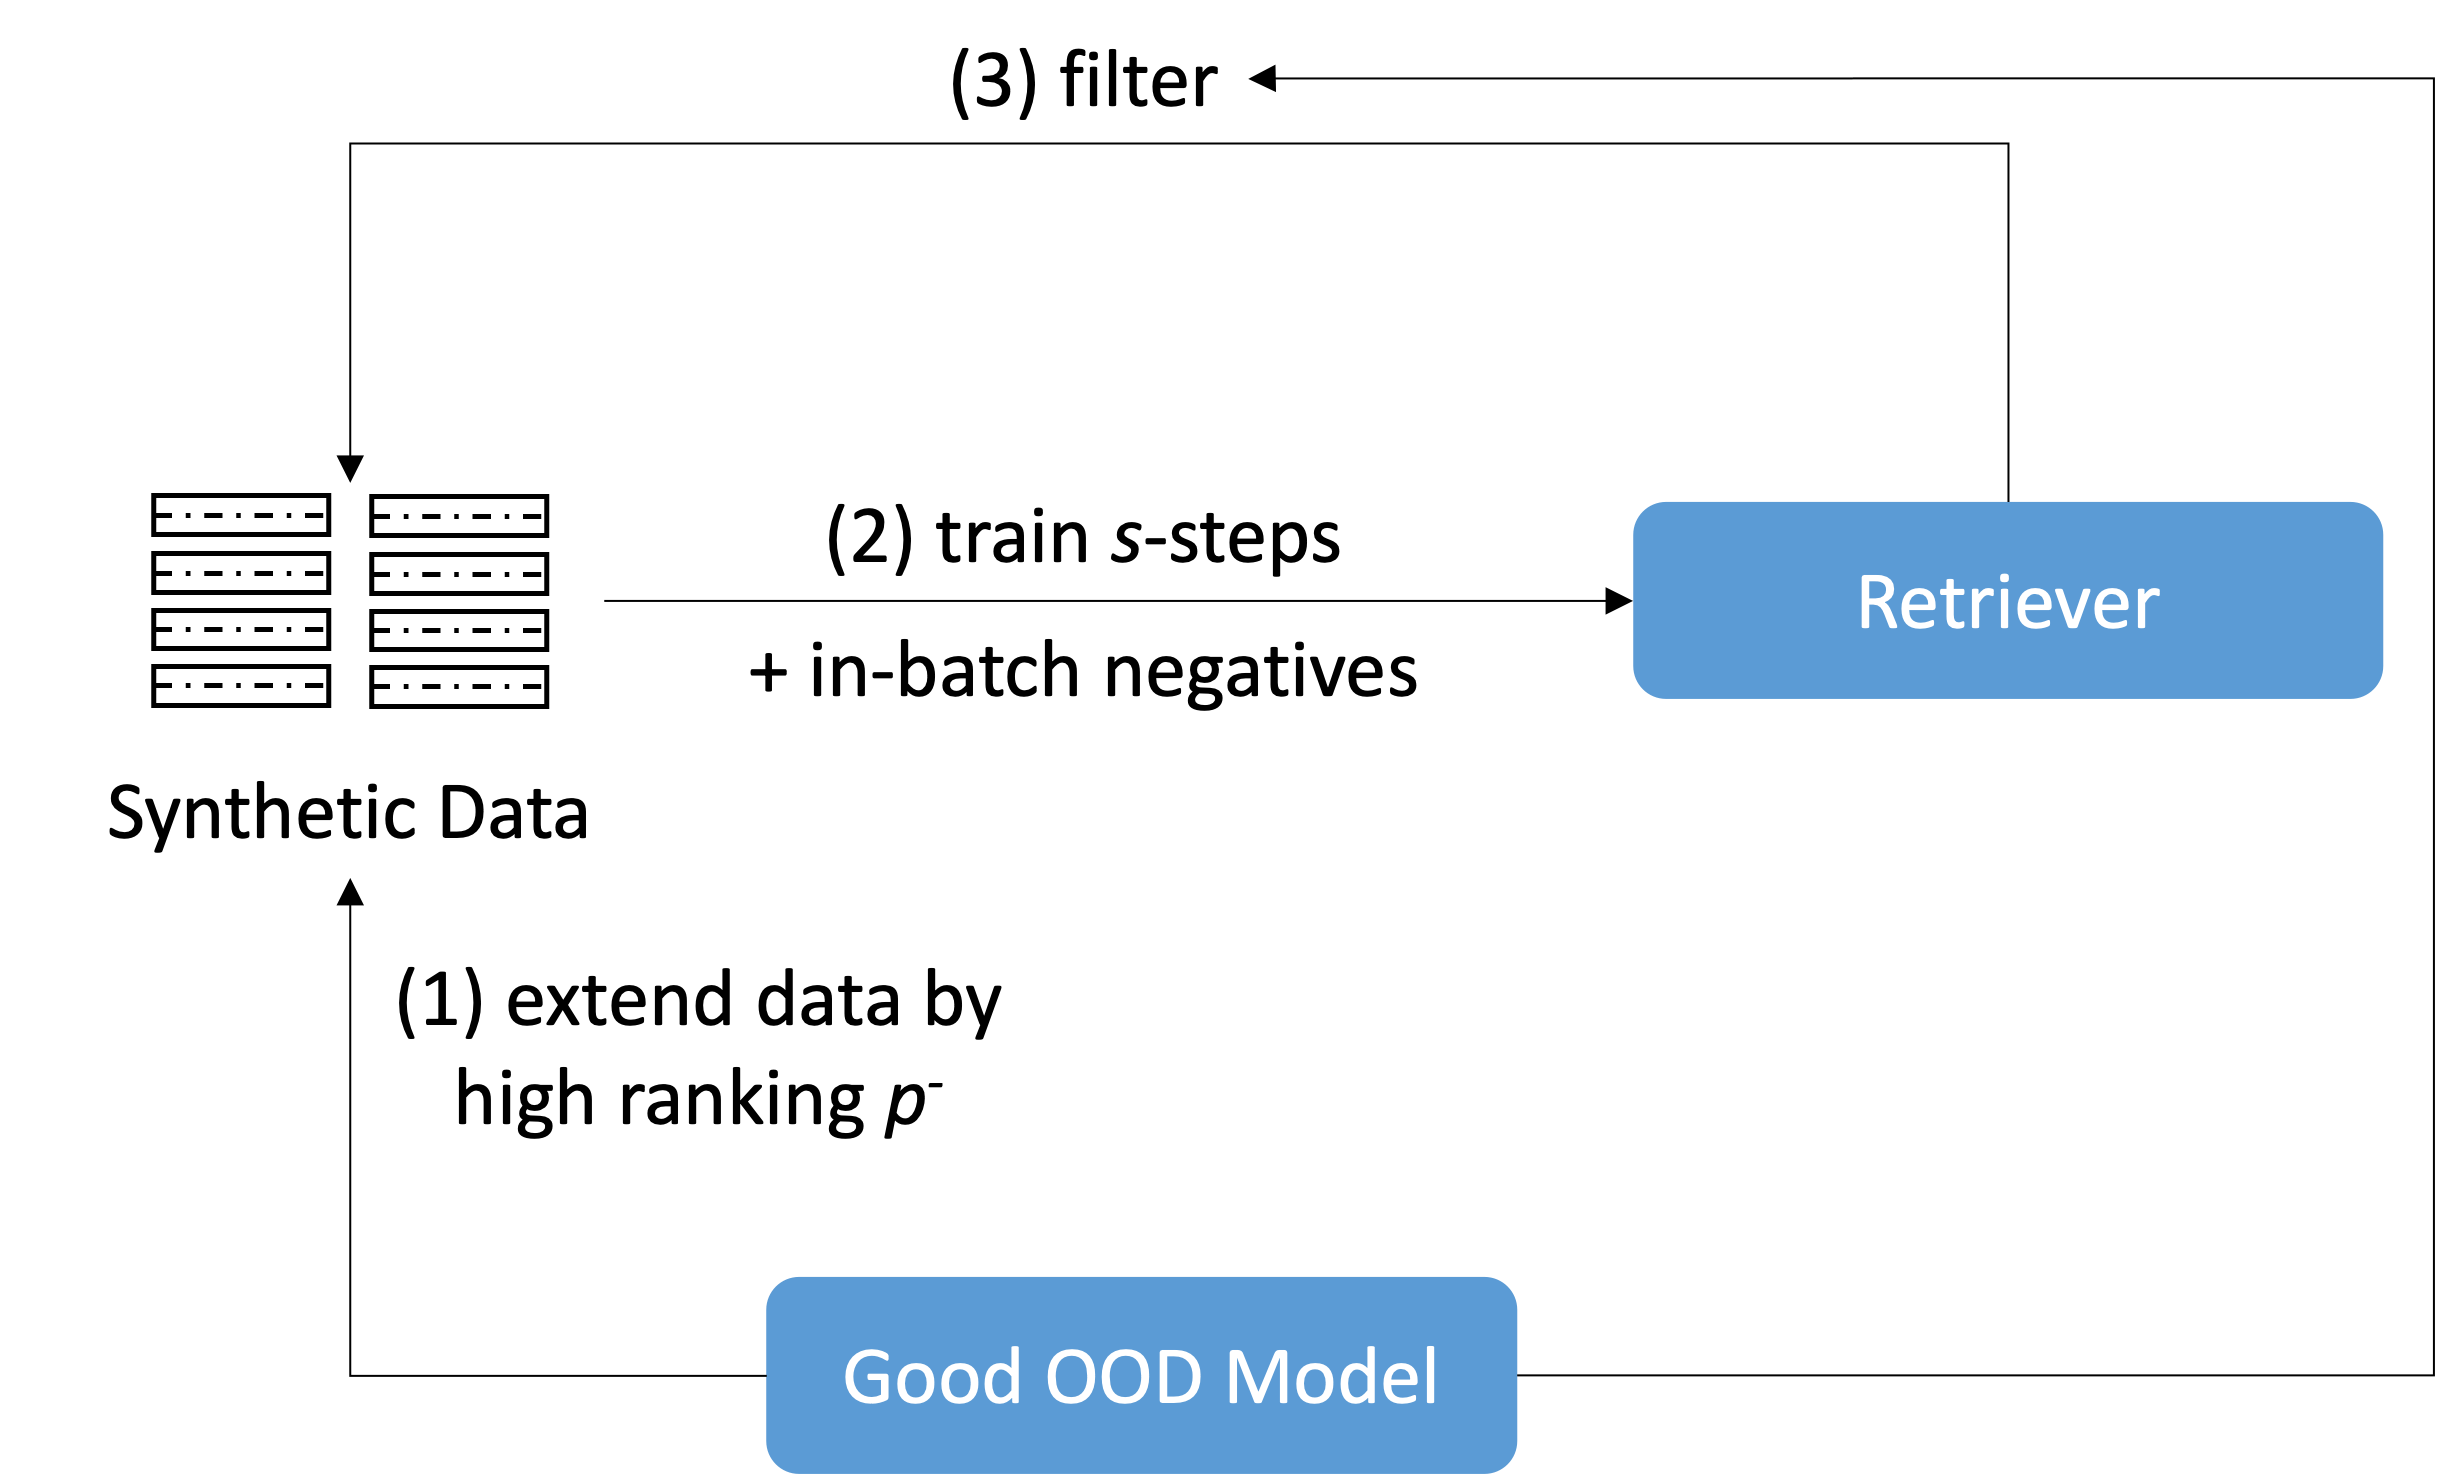
\includegraphics[width=0.8\textwidth]{Grafiken/Training.png}
%     \caption{Fine-Tuning Process for Retriever}
%     \label{fig:retriever-fine-tuning} 
% \end{figure}

% A crucial aspect of this fine-tuning approach is the utilization of an already well-performing out-of-domain retriever as a baseline. This baseline retriever can distill its knowledge into the retriever undergoing training. For example, \gls{dpr} used BM25, while ColBERTv2 employed MiniLM \cite{wang_multi-passage_2019}, a 22M-parameter Interaction-based retriever. A useful guideline for selecting the model is to consult the BEIR leaderboard.

% In the first step, the \gls{ood} model must retrieve the top $k$ passages, denoted as $p_i$, for each synthetic $(q_s,p^{+})$ pair. To generate numerous high-quality negative triples, denoted as $(q_s, p^{+}, p^{-})$, for every retrieved passage $p_i$ (where $p_i \neq p^{+}$), the triple $(q_s, p^{+}, p_i)$ is added to the training dataset.

% In the second step, the target retriever is trained for $s$ iterations. The loss function employed is the negative log likelihood, as defined in Section \ref{subsec:qa_retrieval}. During training, in-batch negatives are utilized. Let $Q$ and $P$ represent the $(B \times d)$ matrices of question and passage embeddings in a batch of size $B$. The matrix $S = Q P^{T}$ contains rows where each corresponds to a question paired with all other passages in the batch. The passages from all the other data points act as negatives for the question $q$.

% In the third step, the synthetic dataset is subjected to filtering. PROMPTAGATOR demonstrated promising results of filtering data by a network trained on the data. For this filtering process, retrieval is performed using both the newly trained model and the \gls{ood} model for a question $q_s$. If neither model retrieves the corresponding passage $p^{+}$ for the synthetic question within their top $k$, that question is removed from the dataset.

% Steps two and three are repeated once during fine-tuning.
% \subsection{Read}
% \label{subsec:read}

% \textbf{Out-of-Domain Readers:} There exists no benchmark for the application of zero-shot or \gls{ood} Readers. As Pereira et. al. \cite{pereira_visconde_2022} point out in their experimental results, the zero-shot performance of \gls{llm}s as Generative Readers is state-of-the-art and thus needs no fine-tuning and can even perform in a zero-shot setting. Luo et. al. \cite{luo_choose_2022} also pointed out, that the \gls{ood} performance of Extractive Readers is higher than the of Generative ones, when it comes to \gls{prlm}. Threfore a good \gls{ood} model choice is UnifiedQA-v2 \cite{khashabi_unifiedqa-v2_2022}, which is based on T5 \cite{raffel_exploring_2023} and was trained on 20 diverse datasets.

% \noindent\textbf{Fine-Tuning Readers:} Extractive Readers depend on datasets of the form $(q, c, a_span)$, whereas $q$ is a question, $c$ the context and $a_span$ an indication of which tokens of $c$ correspond to the desired answer. Similar for Generative Readers, which need $(q, c, a)$ datasets, whreas $a$ is just a text based answer to question $q$. The training process for the reader is easier and more straightforward as for the retriever. Given the already filtered synthetic trainings dataset, this can be used for training of the reader.

% \subsection{Orchestration}
% \label{subsec:qa_orchestration}

% Similar to \gls{r2d2}\cite{fajcik_r2-d2_2021} and LaPraDoR \cite{xu_laprador_2022} and others, an orchestration of retrievers and readers will be adopted in order to achieve highest \gls{ood} performance. This involves the following steps:

% \begin{enumerate}
%     \item \textit{Retrieval:} The $k$-top identified passages $P = \{p_1, p_2, \ldots, p_k\}$ are retrieved for a given question $q$ receive a similarity indication $\text{sim}(q,p_k)$ by the retriever. Next to this score, the BM25 score is calculated $BM25(q,p_k)$. The final score is calculated as the weighting of the similarity by BM25:     $score(q, d) = sim(q, d) \cdot BM25(q, d)$
%     \item \textit{Reader:} As for the Reader two readers will be executed at the same time: An extractive and one generative reader. Both 

% \end{enumerate}


% \section{Conversational Question Answering System}
% \label{sec:conv-qa-system}